%%% LaTeX Template
%%% This template is made for project reports
%%%	You may adjust it to your own needs/purposes
%%%
%%% Copyright: http://www.howtotex.com/
%%% Date: March 2011

%%% Preamble
\documentclass[10pt]{report}	% Article class of KOMA-script with 11pt font and a4 format

\usepackage{color}
\usepackage{framed}
\usepackage{textcomp}
\usepackage{listings}
\usepackage{hyperref}
\usepackage[page]{appendix}
\usepackage{graphicx}
\usepackage{verbatim}
\usepackage{amsmath}
\usepackage{xspace}
%\usepackage{minitoc}
\usepackage{mtcoff}
\usepackage[tt]{titlepic}
\usepackage{array}

\usepackage{sstmacro}

\usepackage[textwidth=6.5in]{geometry}

\definecolor{shadecolor}{rgb}{1,0.8,0.3}
\definecolor{dkgreen}{rgb}{0,0.6,0}
\definecolor{purple}{rgb}{1,0,1}

\newcommand{\todo}[1] {\textcolor{red}{-[#1]-}}

\newcommand{\nodecls}{\inlinecode{node}\xspace}
\newcommand{\topcls}{\inlinecode{topology}\xspace}
\newcommand{\switchid}{\inlinecode{SwitchId}\xspace}
\newcommand{\nodeid}{\inlinecode{NodeId}\xspace}
\newcommand{\evhandler}{\inlinecode{EventHandler}\xspace}
\newcommand{\evscheduler}{\inlinecode{EventScheduler}\xspace}
\newcommand{\evmgr}{\inlinecode{EventManager}\xspace}

\newcommand{\mytilde}{{\raise.17ex\hbox{$\scriptstyle\sim$}}}

\newcommand{\sstmacro}{{SST/\raise.35ex\hbox{macro}}\xspace}
\newcommand{\sprockit}{{SProCKit}\xspace}
\newcommand{\eg}{\textit{e.g.}}

\newcommand{\class}[1]{\textcolor{blue}{#1}}

\newcommand{\func}[1]{\textcolor{purple}{#1}}

\newcommand{\folder}[1]{\textcolor{dkgreen}{#1}}

\newcommand{\aside}[1]{\begin{framed} #1 \end{framed}}

\newcommand{\guikey}[1]{\emph{#1}}

\newcommand{\inlinefile}[1]{{\lstset{basicstyle=\ttfamily,keywordstyle={}}\lstinline$#1$}}

\newcommand{\inlinecode}[1]{{\lstset{basicstyle=\ttfamily,keywordstyle={},showstringspaces=false}\lstinline$#1$}}
\newcommand{\inlineshell}[1]{{\lstset{basicstyle=\ttfamily,keywordstyle={},showstringspaces=false}\lstinline$#1$}}

\title{SST/macro 12.1: Developer's Reference}

\author{Sandia National Labs \\ Livermore, CA}

\titlepic{
\includegraphics[width=0.3\textwidth]{figures/sstlogo.png}}

\setlength{\parindent}{0cm} % Default is 15pt.
\setlength{\parskip}{2mm plus1mm minus1mm}

\begin{document}

\maketitle 

\tableofcontents

% !TEX root = developer.tex

\chapter{Introduction}\label{chapter:intro}

\section{Overview}
\label{sec:intro:overview}

The \sstmacro software package provides a simulator for large-scale parallel computer architectures.
\sstmacro is a component within the Structural Simulation Toolkit (SST).
SST itself provides the abstract discrete event interface.
\sstmacro implements specifically a coarse-grained simulator for distributed-memory applications. 

The simulator is driven from either a trace file or skeleton application. 
Simulation can be broadly categorized as either off-line or on-line.
Off-line simulators typically first run a full parallel application on a real machine,
recording certain communication and computation events to a simulation trace.
This event trace can then be replayed post-mortem in the simulator.

For large, system-level experiments with thousands of network endpoints, high-accuracy cycle-accurate simulation is not possible,
or at least not convenient.
Simulation requires coarse-grained approximations to be practical.
\sstmacro is therefore designed for specific cost/accuracy tradeoffs.

The developer's manual broadly covers the two main aspects of creating new components.
\begin{itemize}
\item Setting up components to match the \inlinecode{Connectable} interface linking components together via ports and event handlers
\item Registering components with the factory system to make them usable in simulation input files
\end{itemize}

\section{What To Expect In The Developer's Manual}
\label{sec:whatToExpect}

The developer's manual is mainly designed for those who wish to extend the simulator or understand its internals.
The user's manual, in contrast, is mainly designed for those who wish to perform experiments with \emph{new} applications using \emph{existing} hardware models.
The user's manual therefore covers building and running the core set of SST/macro features.
The developer's manual covers what you need to know to add new features.
The SST design is such that external components are built into shared object \inlinecode{.so} files,
loading them into the simulator core without having to recompile the core itself.

\section{Thousand Foot View of Discrete Event Simulation}
\label{sec:thousandFoot}

Ignoring the complexities of parallel discrete event simulation (PDES), 
discrete even simulation works with a very simple set of abstractions.
Implementing a discrete event simulation requires components, links, and events (Figure~\ref{fig:desCore}).
Components (or agents) perform operations. Components create, send, and receive events - and that's basically all they do. 
In one example, each component could represent a compute node in the system.
Links between components could represent actual, physical links in the network.
The events sent on links are MPI messages.

Time only advances in the simulator \emph{between} events.
It is important to distinguish virtual time (the time being estimated by simulation) from wall clock time (the real time the simulator is running).
Links have an associated latency (delay) and are scheduled by the simulation core to arrive at components at a specific time.
This list of event arrivals at components creates an event queue (more precisely event heap) that is sorted by soonest event time.
As events are popped off the heap, the simulation clock is updated.
The component handles the incoming event, which could cause the component to create and send new events to other components.
The simulation ends when all components quiesce, with no more events active in the system.

Components never interact directly (i.e. a component can never have a shared-memory pointer to another component).
Components can only interact with links.
All information transmitted between components must be encapsulated as an abstract event.
In parallel discrete event simulation, the challenge is both delivering events through distributed memory and maintaining a consistent virtual clock.
Without proper synchronization, one component could have its virtual clock advance too quickly.
It then might receive events from other components with timestamps in the past,
creating an event order violation.
As long as developers obey the component, link, and event abstractions, all of these complexities are handled automatically by the simulation core.

\begin{figure}
\centering
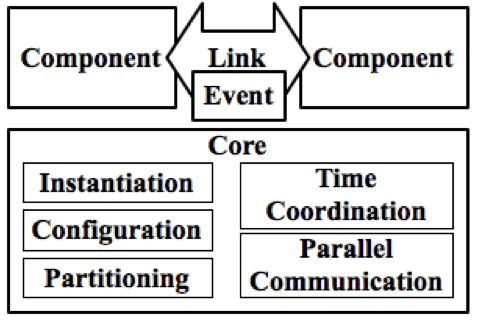
\includegraphics[width=0.3\textwidth]{figures/desCore.png}

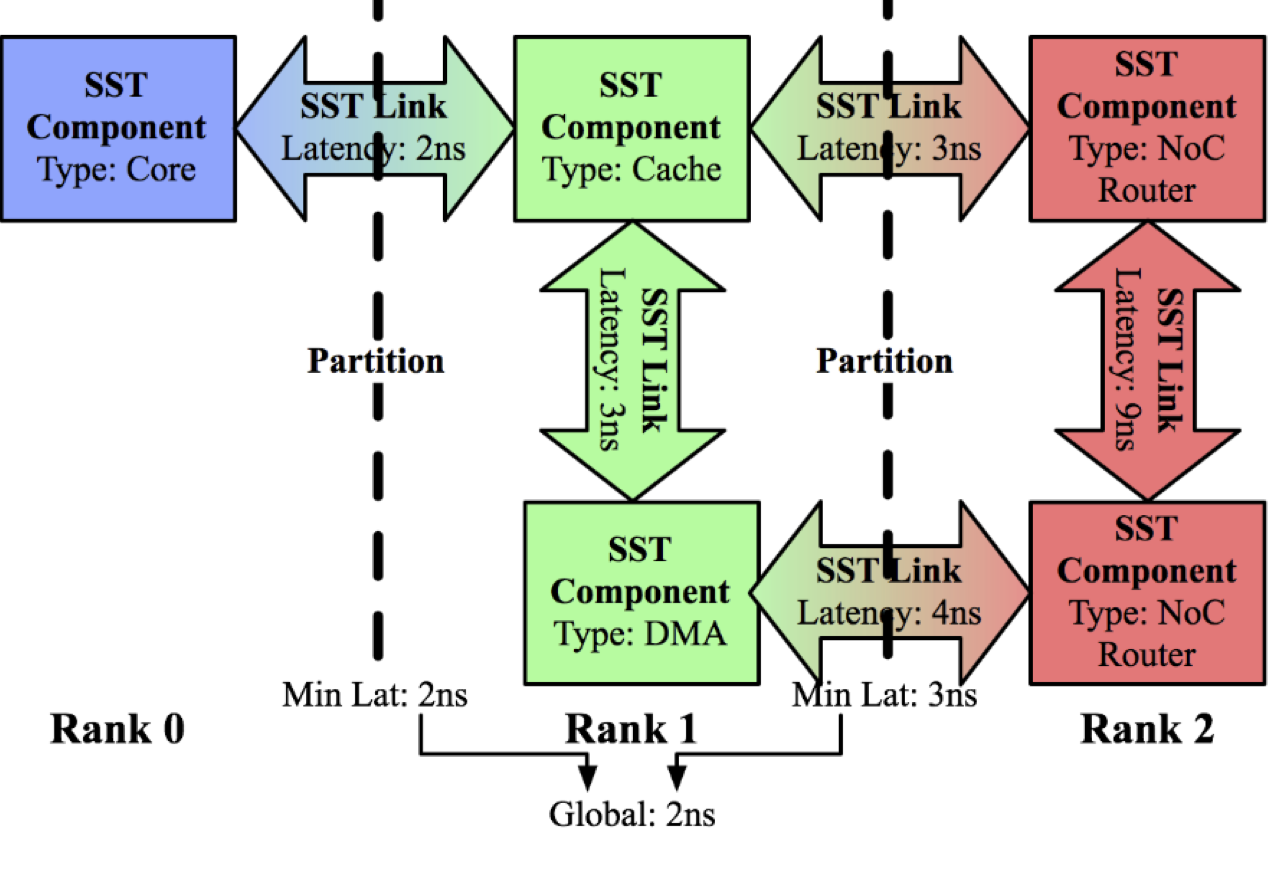
\includegraphics[width=0.5\textwidth]{figures/pdesCore.png}
\caption{Basic structure of discrete event simulation linking components with links (of a given latency). Link delays advance the simulation clock, which is coordinated by the discrete event core. Parallel discrete event simulation involves placing components on different MPI ranks. The link objects (and simulator core) are responsible for delivering events across MPI boundaries.}
\label{fig:desCore}
\end{figure}

\section{Use of C++}
\label{sec:useCpp}

SST/macro (Structural Simulation Toolkit for Macroscale) is a discrete event simulator designed for macroscale (system-level) experiments in HPC. 
SST/macro is an object-oriented C++ code that makes heavy use of dynamic types and polymorphism.
While a great deal of template machinery exists under the hood, nearly all users and even most developers will never actually need to interact with any C++ templates.
Most template wizardry is hidden in easy-to-use macros.
While C++ allows a great deal of flexibility in syntax and code structure, we are striving towards a unified coding style.

Boost is no longer required or even used.
Some C++11 features like \inlinecode{unordered_map} and \inlinecode{unique_ptr} are used heavily throughout the code.

\begin{figure}
\centering
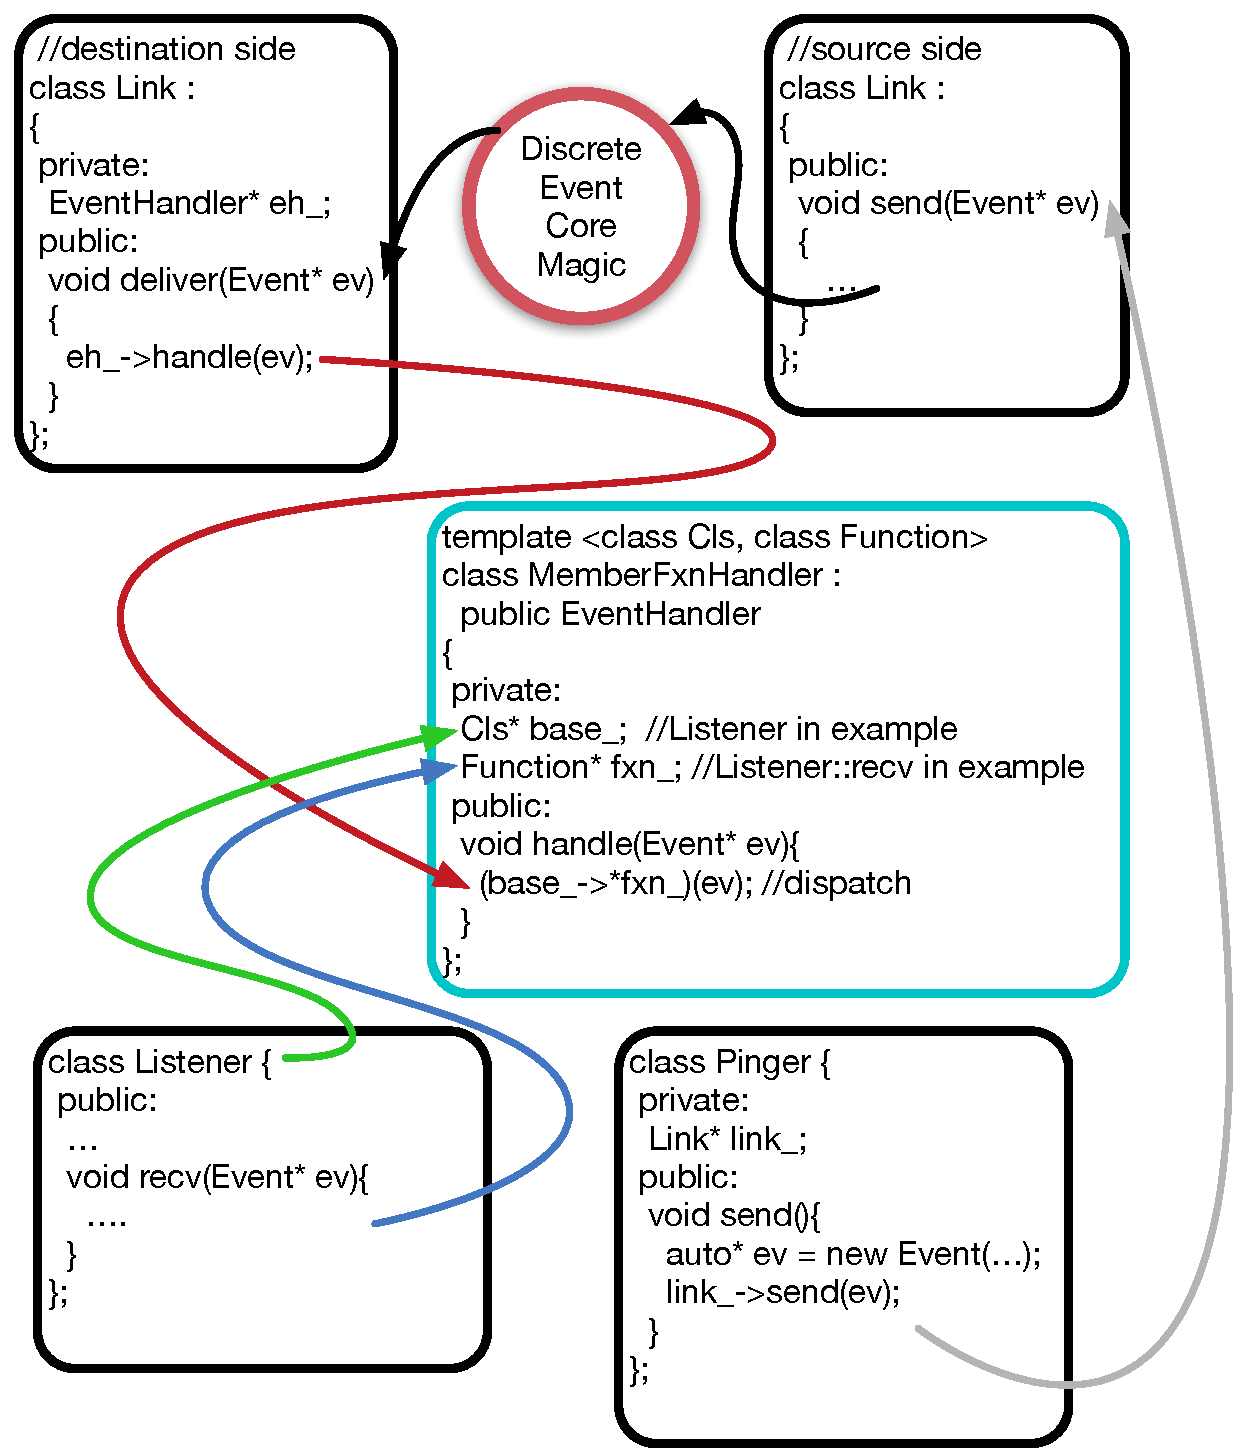
\includegraphics[width=0.8\textwidth]{figures/EventHandler}
\caption{Structure of the simulation connecting components with links and event handlers.}
\label{fig:abstractHandlers}
\end{figure}

\section{Polymorphism and Modularity}
\label{sec:polymorphism}

The simulation progresses with different modules (classes) exchanging events.
In general, when module 1 sends a message to module 2, module 1 only sees an abstract interface for module 2.
The polymorphic type of module 2 can vary freely to employ different physics or congestions models without affecting the implementation of module 1. 
Polymorphism, while greatly simplifying modularity and interchangeability, does have some consequences.
The ``workhorse'' of SST/macro is the base \inlinecode{event}, \inlinecode{Component}, and \inlinecode{EventHandler} classes.
To increase polymorphism and flexibility, every SST/macro module that receives events does so via a generic function

\begin{CppCode}
void handle(Event* ev){
...
}
\end{CppCode}
The prototype therefore accepts \emph{any} event type. 
The interaction of these types is illustrated in Figure~\ref{fig:abstractHandlers}).
Event handlers are created as dispatch wrappers to member functions of a \inlinecode{Component} or \inlinecode{SubComponent}.
There are special helper functions and template classes in SST/macro designed to simplify this process.
A \inlinecode{Link} is created connecting two components.
An \inlinecode{EventHandler} is created that dispatches to the \inlinecode{Listener::recv} member function.
When events are pushed onto the link by \inlinecode{Pinger},
the simulation core computes the correct link delay.
After advancing virtual simulation time,
the simulation core invokes the event handler, which delivers the event to the \inlinecode{Listener}.

Misusing types in SST/macro is \emph{not} a compile-time error.
The onus of correct event types falls on runtime assertions.
All event types may not be valid for a given module.
The other consequence is that a lot of dynamic casts appear in the code.
An abstract \inlinecode{Event} type is received, but must be converted to the specific event type desired.
NOTE: While \emph{some} dynamic casts are sometimes very expensive in C++ (and are implementation-dependent),
most SST/macro dynamic casts are simple equality tests involving virtual table pointers and relatively low overhead.

While, SST/macro strives to be as modular as possible, allowing arbitrary memory, NIC, interconnect components,
in many cases certain physical models are simply not compatible.
For example, using a fluid flow model for memory reads cannot be easily combined with a packet-based model for the network.
Again, pairing incompatible modules is not a compile-time error.
Only when the types are fully defined at runtime can an incompatibility error be detected.

\section{Most Important Style and Coding Rules}
\label{sec:stylerules}

Here is a selection of C++ rules we have tended to follow.
Detailed more below, example scripts are included to reformat the code style however you may prefer for local editing.
However, if committing changes to the repository, only use the default formatting in the example scripts.
\begin{itemize}
\item CapitalCase is use for class names
\item camelCase is used for member function names
\item We use ``one true brace`` style (OTBS) for source files. 
\item In header files, all functions are inline style with attached brackets.
\item To keep code compact horizontally, indent is set to two spaces. Namespaces are not indented.
\item Generally, all if-else and for-loops have brackets even if a single line.
\item Accessor functions are not prefixed, i.e. a function would be called \inlinecode{name()} not \inlinecode{getName()}, except
where conflicts require a prefix. Functions for modifying variables are prefixed with \inlinecode{setX},
\item We use .h and .cc instead of .hpp and .cpp
\item As much implementation as possible should go in .cc files.
	Header files can end up in long dependency lists in the make system.  
	Small changes to header files can result in long recompiles.
	If the function is more than a basic set/get, put it into a .cc file.
\item Header files with many classes are discouraged.  When reasonable, one class per header file/source file is preferred.
	 Many short files are better than a few really long ones.
\item Document, document, document.  If it isn't obvious what a function does, add doxygen-compatible documentation.
	Examples are better than abstract wording.
\item Use STL containers for data structures.  Do not worry about performance until much later.
\item Forward declarations.  There are a lot of interrelated classes, often creating circular dependencies. In addition, you can add up with an explosion of include files, often involving classes that are never used in a given \inlineshell{.cc} file.  For cleanliness of compilation, you will find many \inlineshell{*_fwd.h} files throughout the code. If you need a forward declaration, we encourage including this header file rather than ad hoc forward declarations throughout the code.
\end{itemize}

%Since we respect the sensitivity of code-style wars, we include scripts that demonstrate basic usage of the C++ code formatting tool \emph{astyle}.
%This can be downloaded from {http://astyle.sourceforge.net}. 
%A python script called \inlineshell{fix_style} is included in the top-level bin directory.
%It recursively reformats all files in a given directory and its subdirectories.

%\section{Memory Allocation}\label{sec:memalloc}
%To improve performance, custom memory allocation strategies can be employed in C++.
%At present, a global custom \inlinecode{operator new} can be optionally activated which is optimized for large pages and memory pools.
%At present, no class-specific implementation of \inlinecode{operator new} is used.
%However, we may soon implement custom allocation techniques to improve things like cache/TLB efficiency.
%This is the only major change expected to SST/macro that would affect externally developed modules - and even here the expected modifications would be quite small.
%Because custom allocation schemes may be used, all externally developed code should use \inlinecode{operator new}, rather than \emph{not}  \inlinecode{malloc} or \inlinecode{mmap}, unless allocating very large arrays.


% !TEX root = developer.tex

\chapter{\sstmacro Classes}\label{chapter:classes}

\section{Factory Types}\label{sec:factory}
We here introduce factory types, i.e. polymorphic types linked to keywords in the input file.
String parameters are linked to a lookup table, finding a factory that produces the desired type.
In this way, the user can swap in and out C++ classes using just the input file.
There are many distinct factory types relating to the different hardware components.
There are factories for topology, NIC, node, memory, switch, routing algorithm - the list goes on.
Here show how to declare a new factory type and implement various polymorphic instances.
The example files can be found in \inlineshell{tutorials/programming/factories}.

\subsection{Usage}\label{subsec:usage}
Before looking at how to implement factory types, let's look at how they are used.
Here we consider the example of an abstract interface called \inlinecode{Actor}.
The code example is found in \inlineshell{main.cc}. The file begins

\begin{CppCode}
#include <sstmac/skeleton.h>
#include "actor.h"

namespace sstmac {
    namespace tutorial {

int main(int argc, char **argv)
{
\end{CppCode}
The details of declaring and using external apps is found in the user's manual.
Briefly, the \sstmacro compiler wrapper reroutes the main function to be callable within a simulation.
From here it should be apparent that we defined a new application with name \inlinecode{rob_reiner}.
Inside the main function, we create an object of type \inlinecode{Actor}.

\begin{CppCode}
auto actor_name = getParams().find<std::string>("actor_name");
Actor* the_guy = sprockit::create<Actor>(actor_name, getParams());
the_guy->act();
return 0;
\end{CppCode}
Unseen here, there is an \inlinecode{Actor} factory called via the \inlinecode{sprockit::create} function to create the object.
The value of \inlineshell{actor_name} is read from the input file \inlineshell{parameters.ini} in the directory.
Depending on the value in the input file, a different type will be created.
The input file contains several parameters related to constructing a machine model - ignore these for now.
The important parameters are:

\begin{ViFile}
node {
 app1 {
  exe = ./runtest
  biggest_fan = jeremy_wilke
  actor_name = patinkin
  sword_hand = right
 }
}
\end{ViFile}

Using the Makefile in the directory, if we compile and run the resulting executable we get the output

\begin{ViFile}
Hello. My name is Inigo Montoya. You killed my father. Prepare to die!
Estimated total runtime of           0.00000000 seconds
SST/macro ran for       0.0025 seconds
\end{ViFile}

If we change the parameters:

\begin{ViFile}
node {
 app1 {
  exe = ./runtest
  biggest_fan = jeremy_wilke
  actor_name = guest
  num_fingers = 6
 }
}
\end{ViFile}

we now get the output

\begin{ViFile}
You've been chasing me your entire life only to fail now.
I think that's the worst thing I've ever heard. How marvelous.
Estimated total runtime of           0.00000000 seconds
SST/macro ran for       0.0025 seconds
\end{ViFile}

Changing the values produces a different class type and different behavior.
Thus we can manage polymorphic types by changing the input file.

\subsection{Base Class}\label{subsec:baseClass}
To declare a new factory type, you must include the factory header file

\begin{CppCode}
#include <sprockit/factories/factory.h>

namespace sstmac {
    namespace tutorial {

class Actor {
\end{CppCode}


We now define the public interface for the actor class

\begin{CppCode}
 public:
  Actor(SST::Params& params);
  
  virtual void act() = 0;

  virtual ~actor(){}
\end{CppCode}
Again, we must have a public, virtual destructor.
Each instance of the \inlinecode{Actor} class must implement the \inlinecode{act} method.

For factory types, each class must take a parameter object in the constructor.
The parent class has a single member variable

\begin{CppCode}
 protected:
  std::string biggest_fan_;
\end{CppCode}

Inside the class, we need to register and describe the base type to SST.

\begin{CppCode}
  SST_ELI_DECLARE_BASE(Actor)
  SST_ELI_DECLARE_DEFAULT_INFO()
  SST_ELI_DECLARE_CTOR(SST::Params&)
\end{CppCode}
In almost all cases, only the default info is needed.

Moving to the \inlineshell{actor.cc} file, we see the implementation

\begin{CppCode}
namespace sstmac {
    namespace tutorial {

Actor::Actor(SST::Params& params)
{
  biggest_fan_ = params.find<std::string>("biggest_fan");
}
\end{CppCode}
We initialize the member variable from the parameter object.  

\subsection{Child Class}\label{subsec:childClass}
Let's now look at a fully implemented, complete \inlinecode{Actor} type.  We declare it

\begin{CppCode}
#include "actor.h"

namespace sstmac {
    namespace tutorial {

class MandyPatinkin :
    public Actor
{
 public:
   MandyPatinkin(SST::Params& params);
  
   SST_ELI_REGISTER_DERIVED(
    Actor,
    MandyPatinkin,
    "macro",
    "patinkin",
    SST_ELI_ELEMENT_VERSION(1,0,0),
    "He's on one of those shows now... NCIS? CSI?")
\end{CppCode}

We have a single member variable

\begin{CppCode}
 private:
  std::string sword_hand_;
\end{CppCode}

This is a complete type that can be instantiated. 
To create the class we will need the constructor:

\begin{CppCode}
MandyPatinkin(SST::Params& params);
\end{CppCode}

And finally, to satisfy the \inlinecode{actor} public interface, we need

\begin{CppCode}
virtual void act() override;
\end{CppCode}

In the class declaration, we need to invoke the macro \inlinecode{SST_ELI_REGISTER_DERIVED} to register
the new child class type with the given string identifier.
The first argument is the parent base class. 
The second argument is the specific child type.
The third argument is the element library to register into  (in the case macro).
The fourth argument is the string descriptor that will be linked to the type.
Finally, a version declaration and documentation string should be given with a brief description.
We can now implement the constructor:

\begin{CppCode}
MandyPatinkin::MandyPatinkin(SST::Params& params) :
  actor(params)
{
  sword_hand_ = params.find<std::string>("sword_hand");

  if (sword_hand_ == "left"){
    sprockit::abort("I am not left handed!");
  }
  else if (sword_hand_ != "right"){
      spkt_abort_printf(value_error,
          "Invalid hand specified: %s",
          sword_hand_.c_str());
  }
}
\end{CppCode}
The child class must invoke the parent class method. 
Finally, we specify the acting behavior

\begin{CppCode}
void MandyPatinkin::act()
{
    std::cout << "Hello. My name is Inigo Montoya. You killed my father. Prepare to die!"
              << std::endl;
}
\end{CppCode}

Another example \inlineshell{guest.h} and \inlineshell{guest.cc} in the code folder shows the implementation for the second class.


\input{Connectable}
% !TEX root = developer.tex

\chapter{SProCKit}\label{chapter:sprockit}
\sstmacro is largely built on the Sandia Productivity C++ Toolkit (\sprockit),
which is included in the \sstmacro distribution.
Projects developed within the simulator using \sprockit can easily 
move to running the application on real machines while still using the \sprockit infrastructure.
One of the major contributions is reference counted pointer types.
The parameter files and input deck are also part of \sprockit.

\section{Debug}\label{sec:debug}
The goal of the \sprockit debug framework is to be both lightweight and flexible.
The basic problem encountered in \sstmacro development early on was the desire to have very fine-grained control over when and where something prints.
Previously declared debug flags are passed through the \inlinecode{debug_printf} macro.

\begin{CppCode}
debug_printf(sprockit::dbg::mpi,
  "I am MPI rank %d of %d",
  rank, nproc);
\end{CppCode}

The macro checks if the given debug flag is active. 
If so, it executes a \inlinecode{printf} with the given string and arguments.
Debug flags are turned on/off via static calls to

\begin{CppCode}
sprockit::debug::turn_on(sprockit::dbg::mpi);
\end{CppCode}

\sstmacro automatically turns on the appropriate debug flags based on the \inlineshell{-d} command line flag
or the \inlineshell{debug = } parameter in the input file.

Multiple debug flags can be specified via OR statements to activate a print statement through multiple different flags.

\begin{CppCode}
using namespace sprockit;
debug_printf(dbg::mpi | dbg::job_launch,
  "I am MPI rank %d of %d",
  rank, nproc);
\end{CppCode}

Now the print statement is active if either MPI or job launching is going to be debugged.

In \inlineshell{sprockit/debug.h} a set of macros are defined to facilitate the declaration.
To create new debug flags, there are two macros.
The first, \inlinecode{DeclareDebugSlot}, generally goes in the header file to make the flag visible to all files.
The second, \inlinecode{RegisterDebugSlot}, goes in a source file and creates the symbols and linkage for the flag.

\begin{CppCode}
launch.h:
DeclareDebugSlot(job_launch);

launch.cc
RegisterDebugSlot(job_launch);
\end{CppCode}

\section{Serialization}\label{sec:serialize}
Internally, \sstmacro makes heavy use of object serialization/deserialization in order to run in parallel with MPI.
To create a serialization archive, the code is illustrated below. Suppose we have a set of variables

\begin{CppCode}
struct point {
 int x;
 int y;
}
point pt;
pt.x = 0;
pt.y = 2;
int niter = 5;
std::string str = "hello";
\end{CppCode}

We can serialize them to a buffer

\begin{CppCode}
sstmac::serializer ser;
ser.set_mode(sstmac::serializer::PACK);
ser.init(new char[512]);
ser & pt;
ser & niter;
ser & str;
\end{CppCode}
In the current implementation, the buffer must be explicitly given.

To reverse the process for a buffer received over MPI, the code would be

\begin{CppCode}
char* buf = new char[512];
MPI_Recv(buf, ...)
sstmac::serializer;
ser.set_mode(sstmac::serializer::UNPACK);
ser.init(buf);
ser & pt;
ser & niter;
ser & str;
\end{CppCode}

Thus the code for serializing is exactly the same as deserializing. The only change is the mode of the serializer is toggled.
The above code assumes a known buffer size (or buffer of sufficient size).
To serialize unknown sizes, the serializer can also compute the total size first.

\begin{CppCode}
sstmac::serializer ser;
ser.reset();
ser.set_mode(sstmac::serializer::SIZER);
ser & pt;
ser & niter;
ser & str;
int size = ser.sizer.size(); //would be 17 for example above
char* buf = new char[size];
...
\end{CppCode}
The known size can now be used safely in serialization.

The above code only applies to plain-old dataypes and strings.
The serializer also automatically handles STL containers
through the \inlinecode{&} syntax.
To serialize custom objects, a C++ class must implement the serializable interface.

\begin{CppCode}
namespace my_ns {
class MyObject : 
  public sstmac::serializable
{
 ImplementSerializable(my_object)
 ...
 void serialize_order(sstmac::serializer& ser);
 ...
};
}
\end{CppCode}
The serialization interface requires inheritance from \inlinecode{serializable}.
This inheritance forces the object to define a \inlinecode{serialize_order} function.
The macro \inlinecode{ImplementSerializable} inside the class creates a set of necessary functions.
This is essentially a more efficient RTTI, mapping unique integers to a polymorphic type.
The forced inheritance allows more safety checks to ensure types are being set up and used correctly.
All that remains now is defining the \inlinecode{serialize_order} in the source file:

\begin{CppCode}
void MyObject::serialize_order(sstmac::serializer& ser)
{
  ser & my_int_;
  set << my_double_;
  ...
}
\end{CppCode}

For inheritance, only the top-level parent class needs to inherit from \inlinecode{serializable}.

\begin{CppCode}
class ParentObject : 
  public sstmac::serializable
{
...
  void serialize_order(sstmac::serializer& set);
...
};

class MyObject :
  public ParentObject
{
 ImplementSerializable(MyObject)
 ...
 void serialize_order(sstmac::serializer& ser);
 ...
};
\end{CppCode}
In the above code, only \inlinecode{MyObject} can be serialized.
The \inlinecode{ParentObject} is not a full serializable type because no descriptor is registered for it
using the macro \inlinecode{ImplementSerializable}.
Only the child can be serialized and deserialized.
However, the parent class can still contribute variables to the serialization.
In the source file, we would have

\begin{CppCode}
void MyObject::serializer_order(sstmac::serializer& ser)
{
  ParentObject::serialize_order(ser);
  ...
}
\end{CppCode}
The child object should always remember to invoke the parent serialization method.





% !TEX root = developer.tex


\chapter{Discrete Event Simulation}
\label{chapter:des}
There are abundant tutorials on discrete event simulation around the web.
To understand the basic control flow of \sstmacro simulations,
you should consult Section 3.6, Discrete Event Simulation, in the user's manual.
For here, it suffices to simply understand that objects schedule events to run at a specific time.
When an event runs, it can create new events in the future.
A simulation driver gradually progresses time, running events when their time stamp is reached.
As discussed in the user's manual, we must be careful in the vocabulary.
\emph{Simulation time} or \emph{simulated time} is the predicted time discrete events are happening in the simulated hardware.
\emph{Wall time} or \emph{wall clock time} is the time \sstmacro itself has been running.
There are a variety of classes the cooperate in driving the simulation, which we now describe.

\section{Event Managers}
\label{sec:eventManagers}
The driver for simulations is an event manager that provides the function

\begin{CppCode}
virtual void schedule(TimeDelta start_time, Event* event) = 0;
\end{CppCode}
This function must receive events and order them according to timestamp.
Two main types of data structures can be used, which we briefly describe below.

The event manager also needs to provide

\begin{CppCode}
virtual void run() = 0;
\end{CppCode}

The termination condition can be:
\begin{itemize}
\item A termination timestamp is passed.  For example, a simulation might be specified to terminate after 100 simulation seconds. 
Any pending events after 100 seconds are ignored and the simulation exits.
\item The simulation runs out of events.  With nothing left to do, the simulation exits.
\end{itemize}

Events are stored in a queue (sorted by time)

\begin{CppCode}
namespace sstmac {

class ExecutionEvent
{
 public:
  virtual void execute() = 0;

  ...
};
\end{CppCode}

The execute function is invoked by the \evmgr to run the underlying event.
There are generally two basic event types in \sstmacro, which we now introduce.

\subsection{Event Handlers}
\label{subsec:eventHandlers}
In most cases, the event is represented as an event sent to an object called an \evhandler at a specific simulation time.
In handling the event, the event handlers change their internal state and may cause more events
by scheduling new events at other event handlers (or scheduling messages to itself) at a future time.

In most cases, events are created by calling the function

\begin{CppCode}
auto* ev = newCallback(this, &Actor::act);
\end{CppCode}

This then creates a class of type \inlinecode{ExecutionEvent}, for which the execute function is

\begin{CppCode}
template <int ...S> void dispatch(seq<S...>){
  (obj_->*fxn_)(std::get<S>(params_)...);
}

Fxn fxn_;
Cls* obj_;
std::tuple<Args...> params_;
\end{CppCode}

For example, given a class \inlinecode{Actor} with the member function \inlinecode{act}

\begin{CppCode}
void Actor::Actor(Event* ev, int ev_id){...}
\end{CppCode}
we can create an event handler

\begin{CppCode}
Actor* a = ....;
auto* ev = newCallback(a, &actor::act, 42);
schedule(time, , ev);
\end{CppCode}
When the time arrives for the event, the member function will be invoked

\begin{CppCode}
a->act(42);
\end{CppCode}


\subsection{Event Heap/Map}
\label{subsec:eventHeap}
The major distinction between different event containers is the data structured used.
The simplest data structure is an event heap or ordered event map.
The event manager needs to always be processing the minimum event time, which maps naturally onto a min-heap structure.
Insertion and removal are therefore log(N) operations where N is the number of currently scheduled events.
For most cases, the number and length of events is such that the min-heap is fine.

\section{Event Schedulers}
\label{sec:eventSchedulers}
The simulation is partitioned into objects that are capable of scheduling events.
Common examples of \evscheduler objects are nodes, NICs, memory systems, or the operating system.
In serial runs, an event scheduler is essentially just a wrapper for the \evmgr and the class is not strictly necessary.
There are two types of event scheduler: \inlinecode{Component} and \inlinecode{SubComponent}.
In parallel simulation, though, the simulation must be partitioned into different scheduling units.
Scheduling units are then distributed amongst the parallel processes.
Components are the basic unit.  Currently only nodes and network switches are components.
All other devices (NIC, memory, OS) are subcomponents that must be linked to a parent component.
Even though components and subcomponents can both schedule events (both inherit from \evscheduler),
all subcomponents must belong to a component.  A subcomponent cannot be separated from its parent component during parallel simulation.



	
% !TEX root = developer.tex

\chapter{Software Models}
\label{chapter:software}

The driver for most simulations is a skeleton application.
Although this can be arbitrary source code, we will consider the example of an MPI application below.
We will discuss distributed services in Section \ref{sec:distService} below, which is similar to an application.  In general, when we refer to applications we mean scientific codes or client codes that are doing ``domain-specific'' work.  These will be different from service applications like parallel file systems.

We will be very specific with the use of the terms ``virtual'' and ``real'' or ``physical''.
Virtual refers to anything being modeled in the simulator.
Real or physical refers to actual processes running on a host system.
When referring to a skeleton application in the simulator, we refer only to virtual MPI \emph{ranks}.
The term \emph{process} only applies to physical MPI ranks since virtual MPI ranks are not true processes, 
but rather a user-space thread.
Many virtual MPI ranks can be colocated within the same process. A physical process generally has:
\begin{itemize}
\item A heap
\item A stack
\item A data segment (global variable storage)
\end{itemize}

As much as possible, SST/macro strives to make writing skeleton app source code the same as writing source for an actual production application.
All virtual MPI ranks can share the same heap within a process.
There is no strict requirement that each virtual MPI rank have its own contiguous heap.
Rather than make each MPI stack a full pthread, each MPI rank is created as a lightweight user-space thread.
In the simulation, all virtual MPI ranks will be running ``concurrently'' but not necessarily in ``parallel."
Each MPI rank within a process must time-share the process,
meaning the simulator core will context switch between each MPI stack to gradually make forward progress.
While the heap and stack are easy to provide for each virtual MPI rank,
there is no easy way to provide a unique global variable segment to each MPI rank.
This therefore requires the Clang source-to-source compiler to redirect all global variable accesses to user-space thread specific locations.

\section{Applications and User-space Threads}
\label{sec:appThreads}

In a standard discrete event simulation (DES), you have only components and events.
Components send events to other components, which may in turn create and send more events.
Each event has an arrival time associated with it.
Components must process events in time-order and keep a sorted queue of events.
Time advances in the simulation as components pop off and process events from the queue.

SST/macro mixes two modes of advancing time.
The simulator has node, NIC, router, and memory models that advance ``hardware time'' in the standard way.
Applications are not a regular DES component.
They are just a stack and a heap, without an event queue or \inlinecode{handle(event* ev)} callback functions.
Applications just step through instructions, executing to the end of the application.
To advance time, applications must \emph{block} and \emph{unblock}.
In DES, time does not advance \emph{during} events - only between events.
For applications, time does not advance while the application is executing.
It advances between a block/unblock pair.
This is clearly somewhat counterintuitive (time advances while an application is not executing).

The details of block/unblock should never be apparent in the skeleton code.
A skeleton MPI code for SST/macro should \emph{look} exactly like a real MPI code.
To advance time, certain function calls must be intercepted by SST/macro.
This is done through a combination of compile-time/linker-time tricks.
All skeleton apps should be compiled with the \inlineshell{sst++} compiler wrapper installed by SST/macro.
The compiler wrapper sets include paths, includes headers, and directs linkage.

For MPI, this first occurs through include paths. SST/macro installs an \inlineshell{mpi.h} header file.
Thus compiling with \inlineshell{sst++} includes a ``virtual'' MPI header designed for SST.
Next, the MPI header defines macros that redirect MPI calls.

\begin{CppCode}
...
#define MPI_Send(...) sumi::sstmac_mpi()->send(__VA_ARGS__)
...
\end{CppCode}
\inlinecode{sstmac_mpi} is a function we will explore more below.
Inside \inlinecode{MPI_Send}, the SST/macro core takes over.
When necessary, SST/macro will block the active user-space thread and context-switch.

We can illustrate time advancing with a simple \inlinecode{MPI_Send} example.
We have discussed that a user-space thread is allocated for each virtual MPI rank.
The discrete event core, however, still runs on the main application thread (stack).
Generally, the main thread (DES thread) will handle hardware events while the user-space threads will handle software events (this is relaxed in some places for optimization purposes).
Figure \ref{fig:desThreadsMPISend}, shows a flow chart for execution of the send.
Operations occurring on the application user-space thread are shaded in blue while operations on the DES thread are shaded in pink.
Function calls do not advance time (shown in black), but scheduling events (shown in green) do advance time.
Again, this is just the nature of discrete event simulation.
The dashed edge shows a block/unblock pair.  
The call to \inlinecode{mpi_api::send} blocks after enqueuing the send operation with the OS.
Virtual time in the simulation therefore advances inside the \inlinecode{MPI_Send} call,
but the details of how this happens are not apparent in the skeleton app.

\begin{figure}
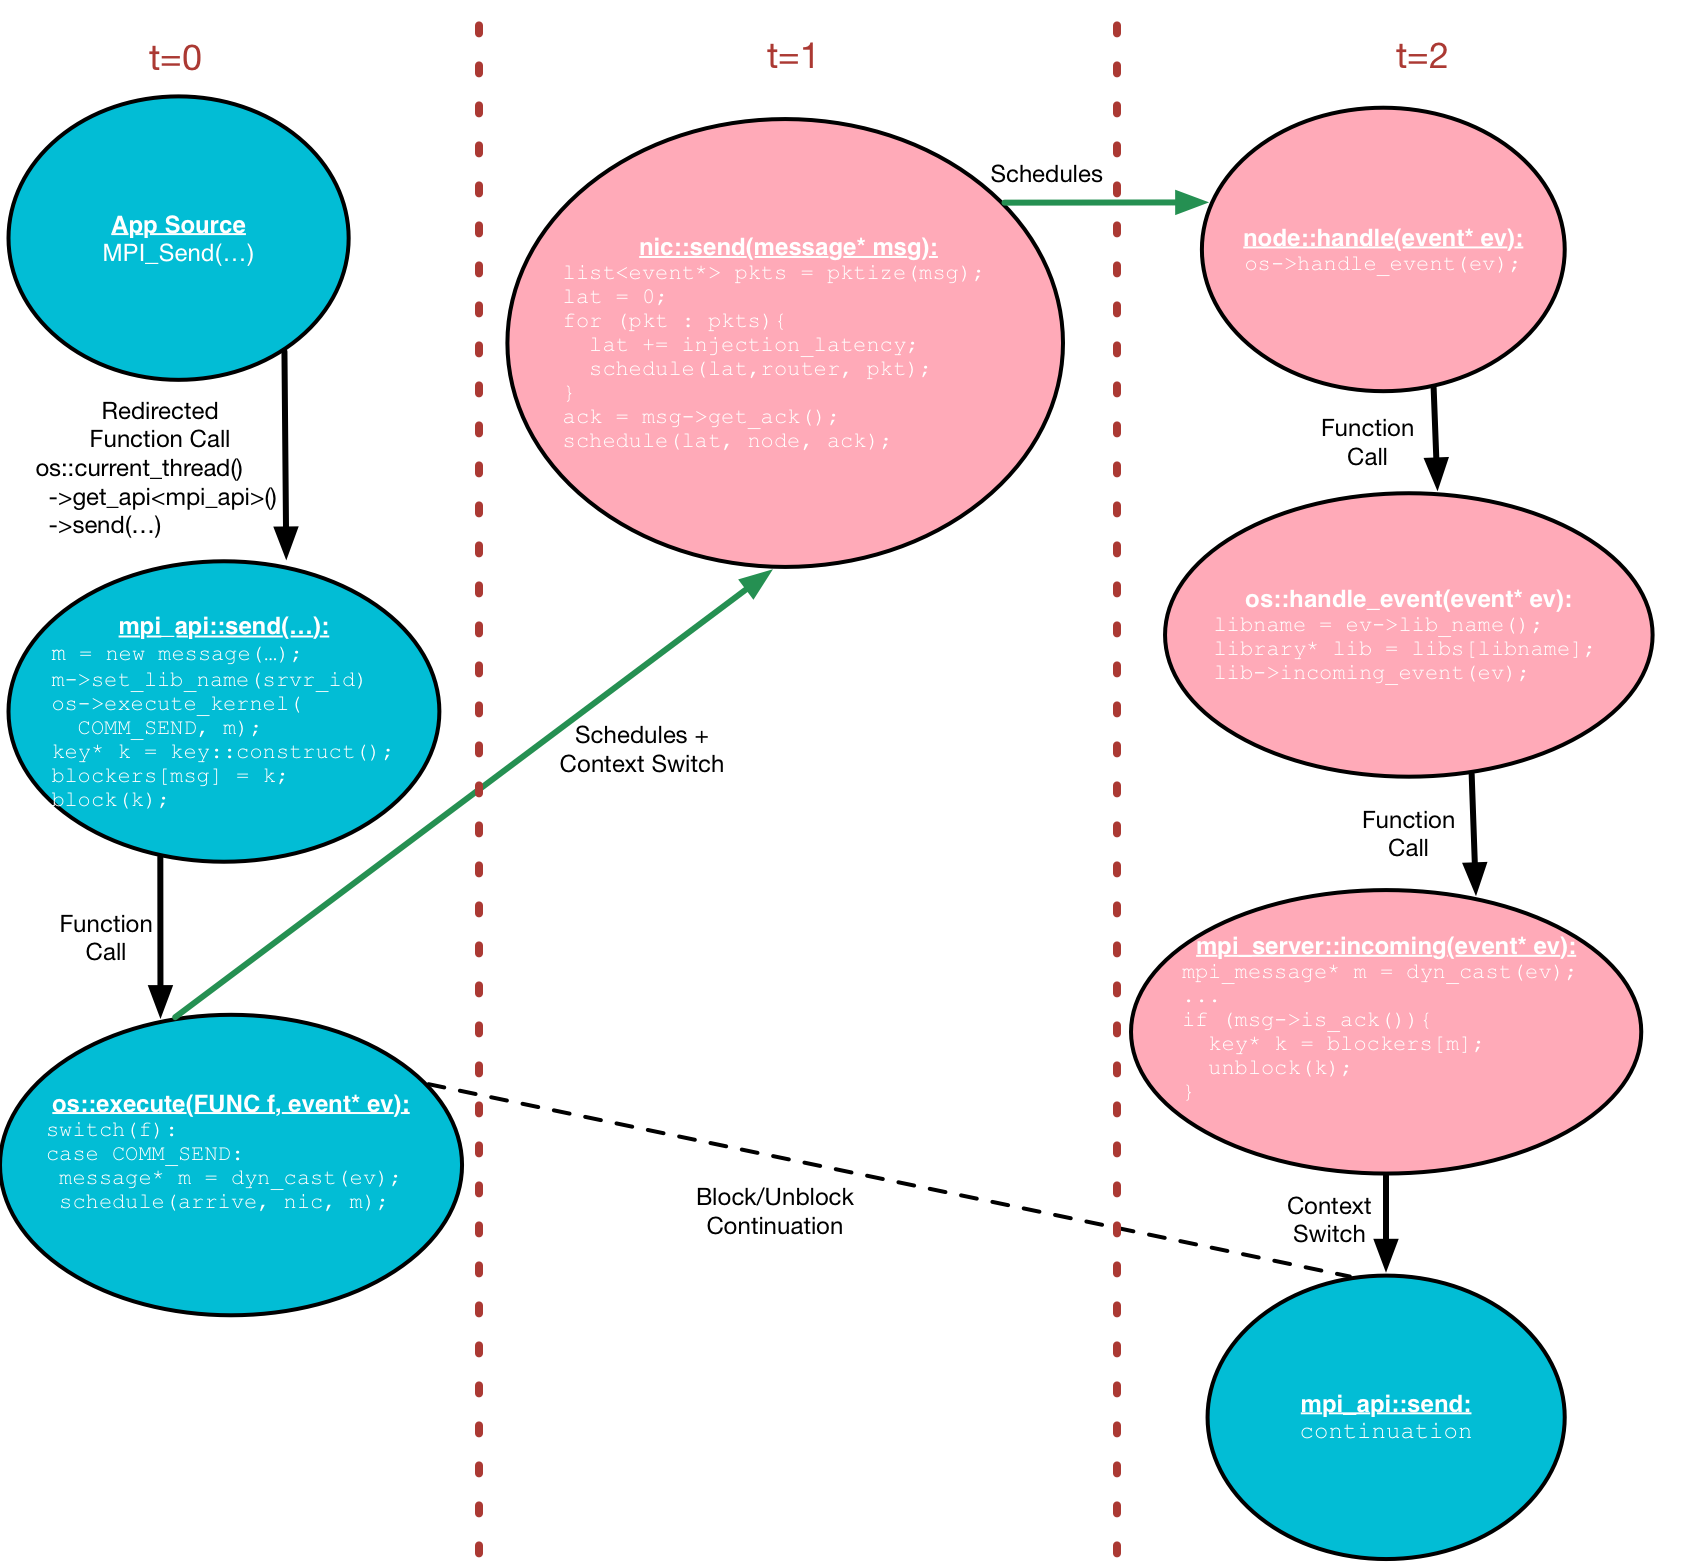
\includegraphics[width=1.05\textwidth]{figures/DES.png}
\caption{Flow of events for completing a send operation.  Shows basic function calls, block/unblock context switches, and event schedules. User-space thread (application) operations are shown in blue. Main event thread (OS/kernel) operations are shown in pink.}
\label{fig:desThreadsMPISend}
\end{figure}

When the ACK arrives back from the NIC, the ACK signals to MPI that the operation is complete allowing it to unblock.
The ACK is handled by a \inlinecode{service} object (which is the SST-specific implementation of an MPI server). 
A \inlinecode{service} is a special type of object, that we will discuss in more detail below.

\subsection{Thread-specific storage}
\label{subsec:threadStorage}
Let us look at the capture of the \inlinecode{MPI_Send} call. 
First, a macro redefines the call to avoid symbol clashes if using an MPI compiler (both virtual and real MPI cannot share symbols).
MPI uses global function calls to execute, meaning MPI has to operate on global variables.
However, SST/macro cannot use global variables.
Thus all state specific to each MPI rank (virtual thread) must be stashed somewhere unique.
This basically means converting all global variables into user-space thread-local variables.
When each user-space thread is spawned a \inlinecode{thread} object is allocated and associated with the thread.
This object acts as a container for holding all state specific to that virtual thread.
Rather than store MPI state in global variables, MPI state in stored in a class \inlinecode{MpiApi}, 
with one \inlinecode{MpiApi} object allocated per virtual MPI rank.
The operating system class provides a static function \inlinecode{currentThread} that makes the leap from
global variables to thread-local storage.
To access a specific API, a special helper template function \inlinecode{getApi} exists on each thread object.
Thus, instead of calling a global function \inlinecode{MPI_Send},
SST/macro redirects to a member function \inlinecode{send} on an \inlinecode{mpi_api} object that is specific to a virtual MPI rank.

\begin{table}
\def\arraystretch{1.5}
\begin{tabular}{>{\raggedright}p{2cm} >{\raggedright}p{3cm} >{\raggedright}p{3cm} >{\raggedright}p{3cm} >{\raggedright\arraybackslash}p{3cm}}
\hline
 & OS & Node & API & Service \\
\hline
Runs on Thread & 
  Both user-space and main DES thread &
  Only main DES thread (user-space with rare exceptions for optimization) &
%  Only main DES thread &
  Only user-space thread &
  Only main DES thread \\
How Advances Time & 
  Both blocking and scheduling events, depending on context &
  Scheduling events to other components &
%  Scheduling events to other components &
  Blocking or unblocking &
  Scheduling events to other components \\
Receives Events Via &
  Function calls from API/Service or from Node via \inlinecode{handle_event} function &
  Function calls from OS, receives scheduled events via the \inlinecode{handle} function &
%  Function calls from Node, receives scheduled events via \inlinecode{handle} function &
  Does not usually receive events - only blocks or unblocks &
  OS forwards messages to \inlinecode{incoming_event} function \\
Sends Events Via &
  Makes function calls and schedules events to Node &
  Makes function calls and schedules events to NIC, Memory &
%  Schedules events to Node, Interconnect &
  Does not usually send events - only blocks or unblocks &
  Makes function calls and schedules events to OS, unblocks APIs
\end{tabular}
\end{table}

\section{Libraries}
\label{sec:libraries}
The creating and handling of software events is managed through \inlinecode{library} objects.
Each \inlinecode{node} has an \inlinecode{OperatingSystem} member variable that will manage software events on a virtual compute node.
Each library object is stored in a lookup table in the operating system,
allowing the operating system to access specific libraries at specific times.

\begin{CppCode}
class OperatingSystem {
  ...
  map<string,Library*> libs_;
  ...
};
\end{CppCode}

Each library object has access to the operating system, being allowed to call

\begin{CppCode}
Event* ev = ...
os_->executeKernel(ty, ev);
\end{CppCode}
where an enum argument \inlinecode{ty} specifies the type of computation or communication and the event object carries all the data needed to model it.
This allows a library to \emph{call out} to the operating system.
Calls to \inlinecode{execute} \emph{always} occur on a user-space thread. 
In executing a computation or communication, the operating system may block inside \emph{execute} to advance time to complete the operation.
Calls to \inlinecode{execute_kernel} can occur on either a user-space thread or the main event thread.
Here the operating system acts as a service and \emph{never} blocks.

Conversely, each \inlinecode{library} must provide a \inlinecode{incomingEvent} method that allows the operating system to call back to the library

\begin{CppCode}
void incomingEvent(event* ev){...}
\end{CppCode}
Generally speaking, event notifications will arrive from the NIC (new messages, ACKs), memory system (data arrived), processor (computation complete), etc.
These hardware events must be routed to the correct software library for processing.

\begin{CppCode}
void OperatingSystem::handleEvent(event* ev) {
  library* lib = libs_[ev->libName()];
  lib->incomingEvent(ev);
}
\end{CppCode}
In order to route events to the correct library, the operating system maintains a string lookup table of \inlinecode{Library} objects.
All events associated with that library must be constructed with the correct string label, 
accessible through the event accessor function \inlinecode{libName}.

\subsection{API}
\label{subsec:softwareAPI}
The SST/macro definition of API was alluded to in \ref{subsec:threadStorage}.
The base \inlinecode{api} class inherits from \inlinecode{library}.
All API code must execute on a user-space thread.
API calls are always associated with a specific virtual MPI rank.
To advance time, API calls must block and unblock.
Functions executing on user-space threads are ``heavyweight'' in the sense that they consume resources.
API compute calls must allocate cores via a compute scheduler to execute.


API objects are accessible in skeleton apps through a global template function is provided in \inlineshell{sstmac/skeleton.h}.

\begin{CppCode}
template <class T>
T* getApi(const std::string& name);
\end{CppCode}
for which the implementation is

\begin{CppCode}
Thread* thr = OperatingSystem::currentThread();
return thr->getApi<T>(const std::string& name);
\end{CppCode}
which converts the global template function into a thread-specific accessor.
The most prominent example of an API is the \inlinecode{MpiApi} object for encapsulating an MPI rank.
Other prominent examples include the various computation APIs such as \inlinecode{BlasApi} that provides bindings for simulation various linear algebra functions.

% !TEX root = developer.tex


\chapter{Hardware Models}
\label{chapter:hardware}

\section{Overview}
\label{sec:topOverview}
To better understand how hardware models are put together for simulating interconnects, we should try to understand the basic flow of event in SST/macro involved in sending a message between two network endpoints.  We have already seen in skeleton applications in previous sections how an application-level call to a function like \inlinecode{MPI_Send} is mapping to an operating system function and finally a hardware-level injection of the message flow.  Overall, the following steps are required:

\begin{itemize}
\item Start message flow with app-level function call
\item Push message onto NIC for send
\item NIC packetizes message and pushes packets on injection switch
\item Packets are routed and traverse the network
\item Packets arrive at destination NIC and are reassembled (potentially out-of-order)
\item Message flow is pushed up network software stack
\end{itemize}

Through the network, packets must move through buffers (waiting for credits) and arbitrate for bandwidth through the switch crossbar and then through the ser/des link on the switch output buffers.  The control-flow diagram for transporting a flow from one endpoint to another via packets is shown in Figure \ref{fig:controlFlow}

In general, sending data across the network (as in, e.g.., MPI), requires the following components:

\begin{itemize}
\item Packetization: handled by \inlinecode{nic} class. Converts flows (MPI messages) into smaller packets.
\item Network topology: handled by \inlinecode{topology} class. Defines the geometry of the network, determining how nodes are connected to switches and how switches are interconnected. It also defines which ports are used for each connection.
\item Fabric management (not yet implemented in SST)
\item Routing: handled by \inlinecode{router} class. Using the defined topology, compute the path that should be taken by a packet. The path is defined by the port numbers that should be taken.
\item Flow control and congestion: handled by \inlinecode{NetworkSwitch} class. Once a path is defined by the router, arbitrate packets (flits) when they contend for bandwidth.
\end{itemize}
As much as possible, these components try to be independent. However, there are inter-dependencies, as shown in Figure \ref{fig:dependencies}.
The router requires topology information to compute paths. For adaptive routing decisions, the router also requires contention information from the network switch.
The network switch requires the computed paths (ports) from the router.

\begin{figure}
\centering
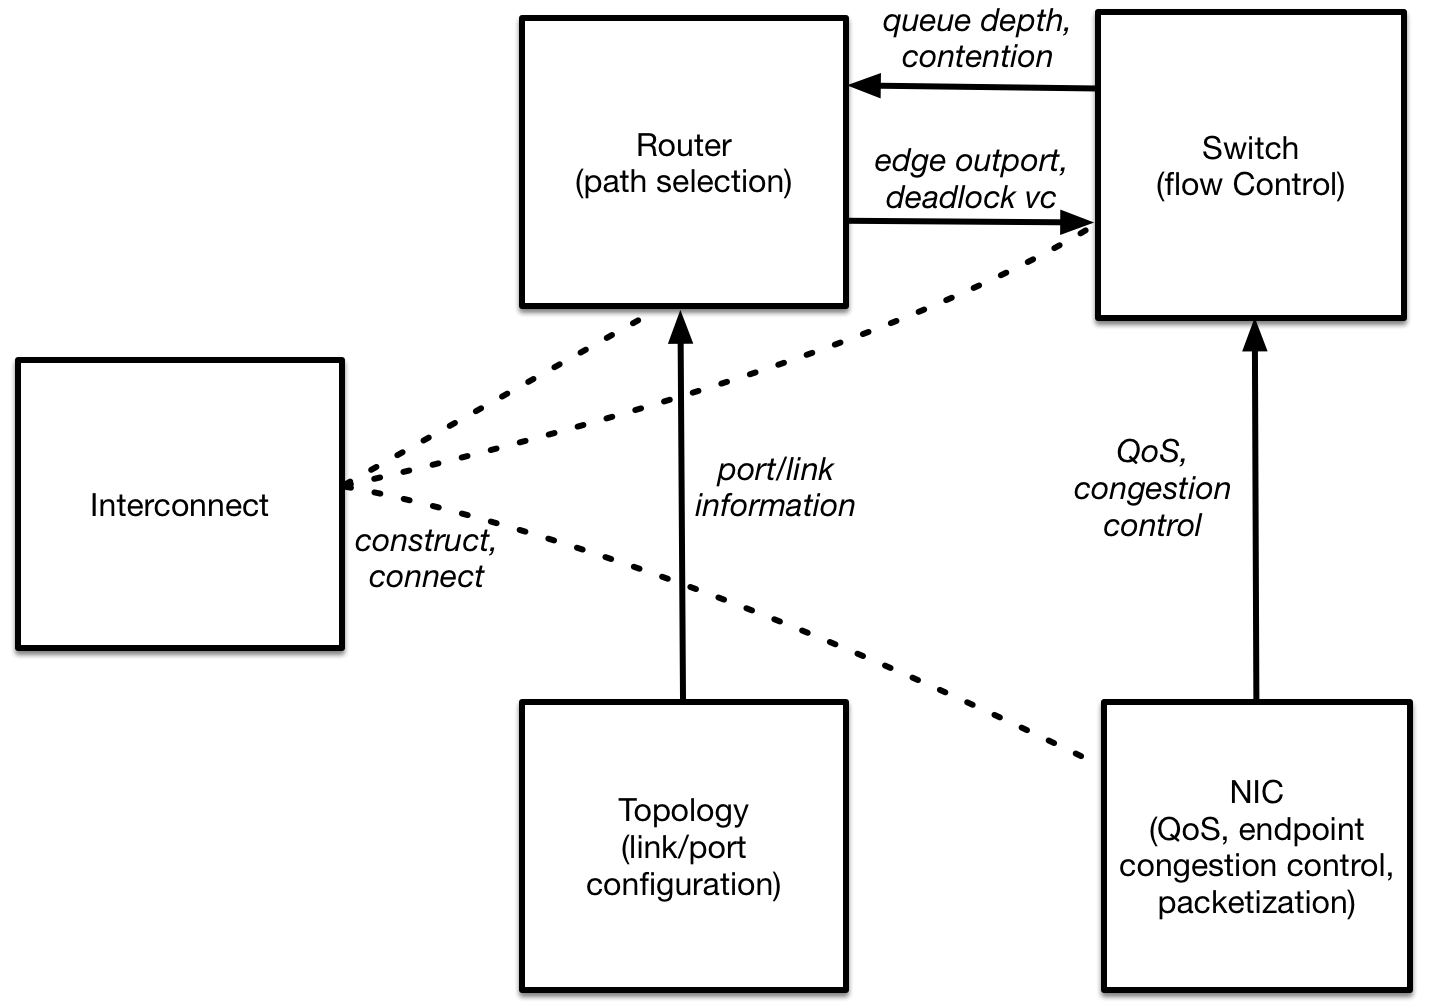
\includegraphics[width=1.0\textwidth]{figures/components.png}
\caption{Components used modeling interconnect and dependencies between them.}
\label{fig:dependencies}
\end{figure}

\begin{figure}
\centering
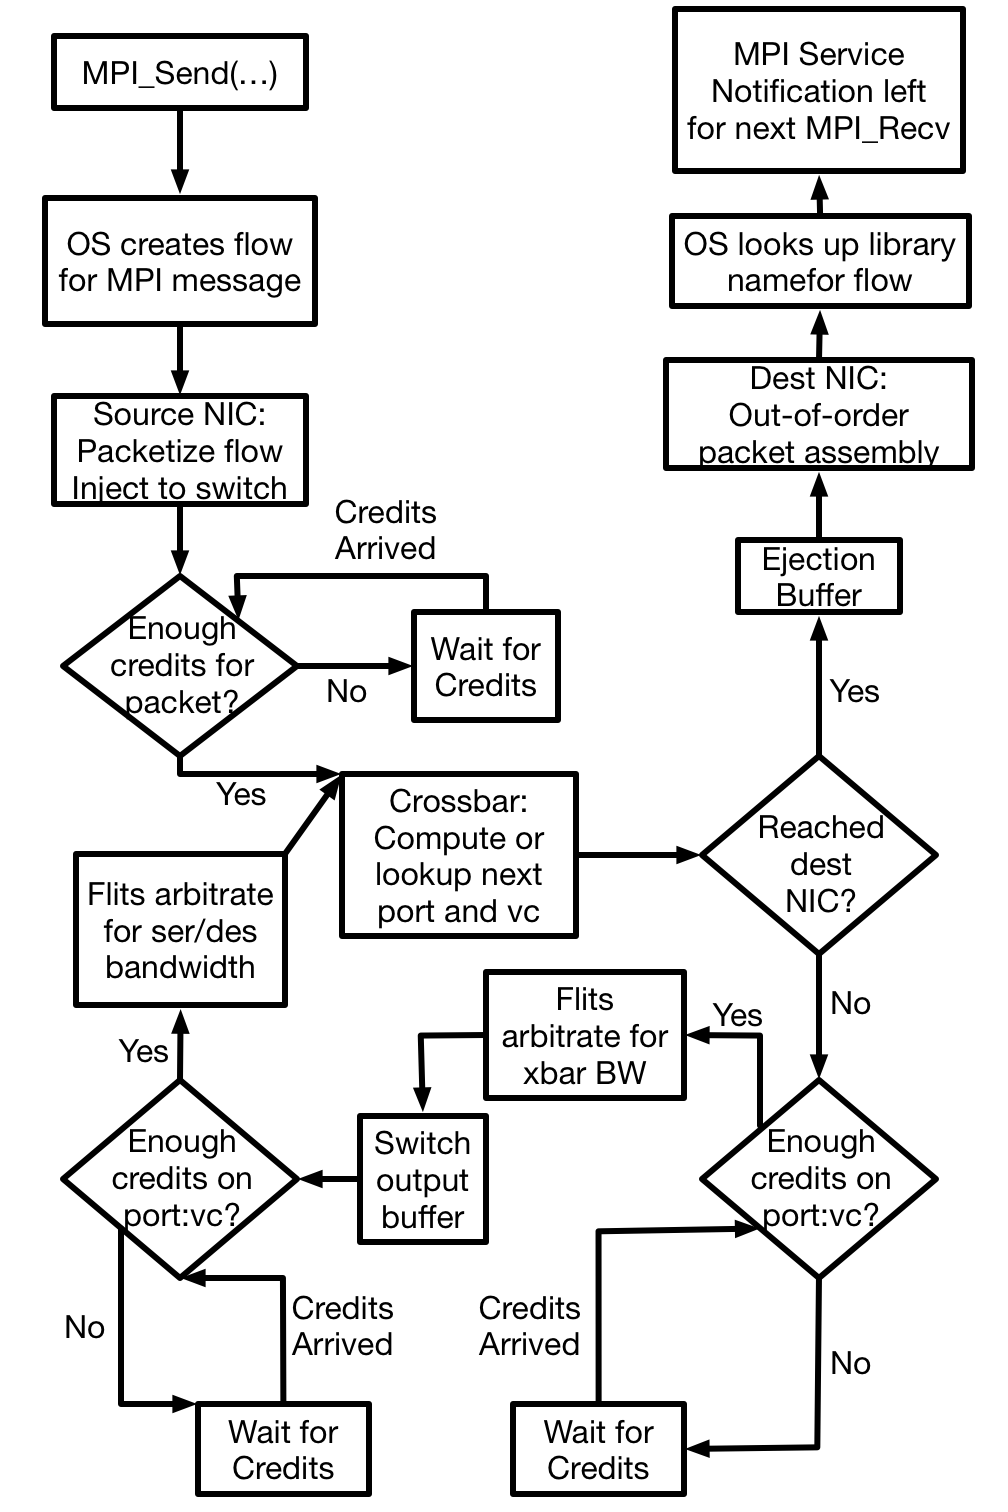
\includegraphics[width=0.75\textwidth]{figures/DecisionFlow.png}
\caption{Decision diagram showing the various control flow operations that occur as a message is transport across the network via individual packet operations.}
\label{fig:controlFlow}
\end{figure}

We can dive in deeper to the operations that occur on an individual component, mos importantly the crossbar on the network switch. Figure \ref{fig:xbarFlow} shows code and program flow for a packet arriving at a network switch.  The packet is routed (virtual function, configurable via input file parameters), credits are allocated to the packet, and finally the packet is arbitrated across the crossbar. After arbitration, a statistics callback can be invoked to collect any performance metrics of interest (congestion, traffic, idle time).

\begin{figure}
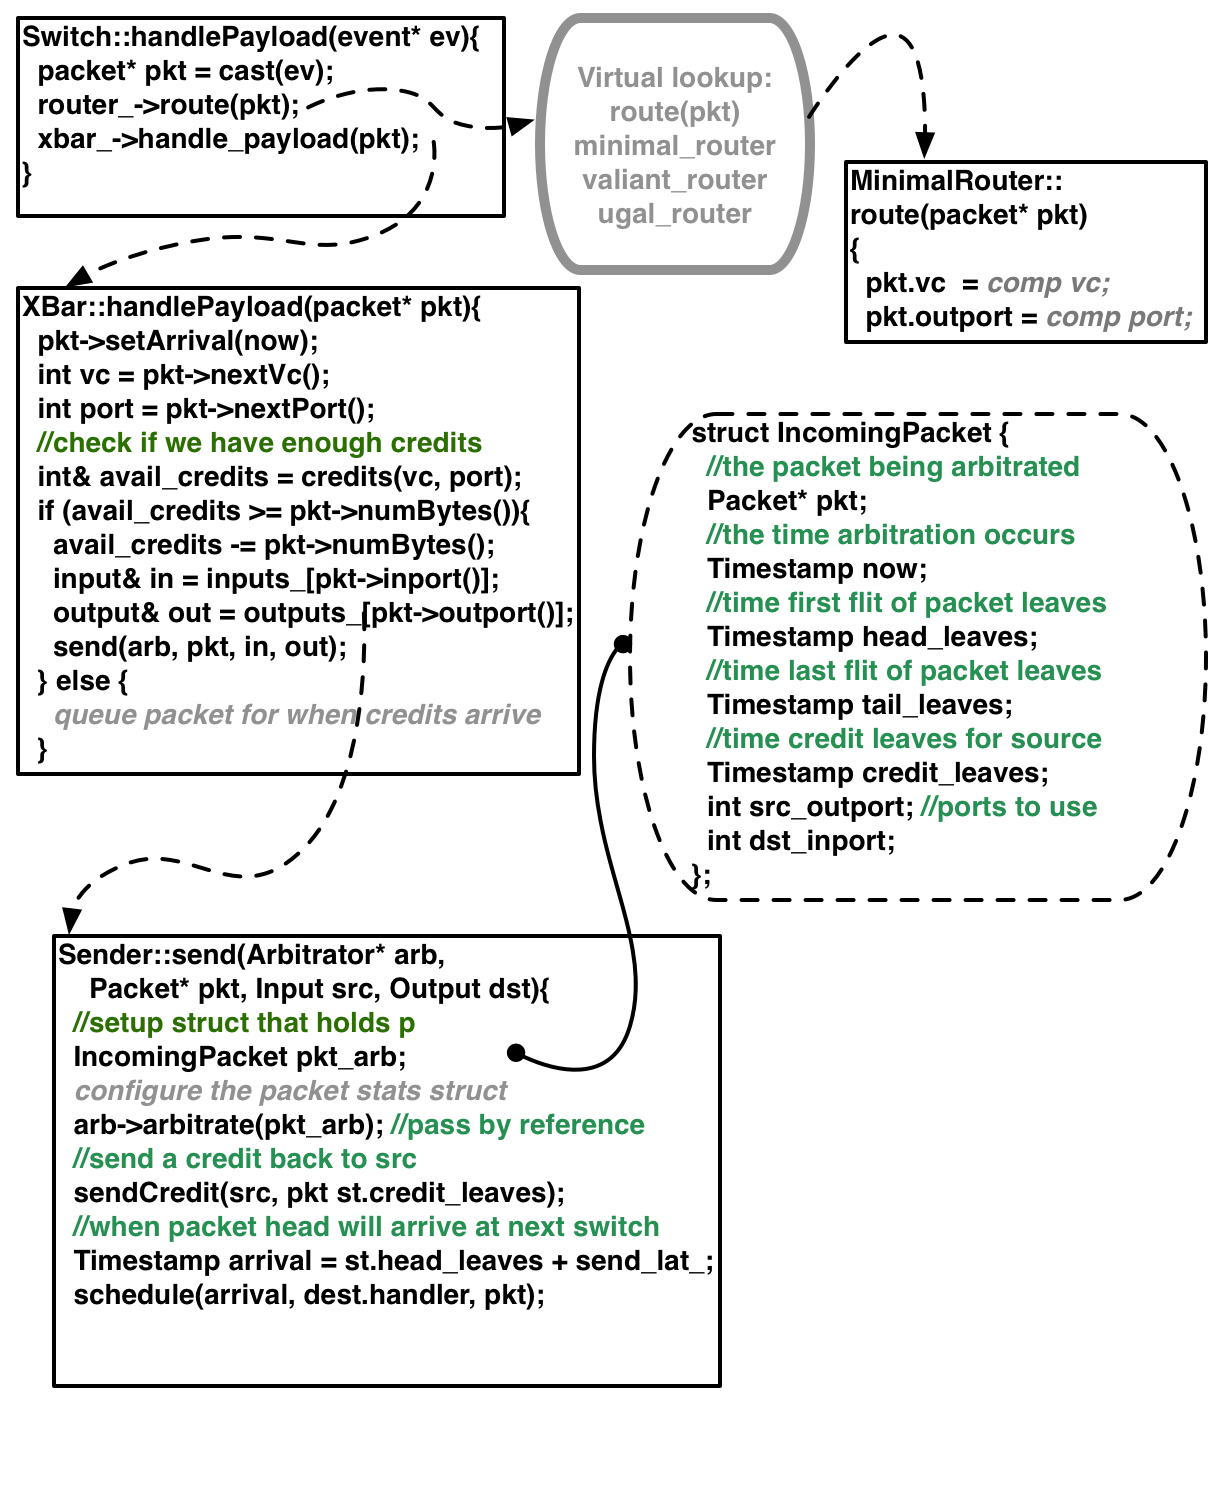
\includegraphics[width=0.9\textwidth]{figures/RoutingFlow.png}
\caption{Code flow for routing and arbitration of packets traversing the crossbar on the network switch.}
\label{fig:xbarFlow}
\end{figure}

\section{Packets}
\label{sec:packets}

Packet must hold information for endpoint control on the NIC, routing decisions, and flow control. 
Packets therefore suffer from a ``combinatorial explosion'' depending on which NIC model is coupled with which flow control mechanism and which routing algorithm.
For example, the simulator is intended to support at least two different network contention models (PISCES, SCULPIN);
five different topologies (torus, hyperX, fat tree, dragonfly, cascade); and four different routing algorithms (Minimal, Valiant, UGAL, PAR).
This creates already 40 combinations, which can grow even more quickly if new models are added.
If the C++ type of the packet were to depend on all of these, messy multiple inheritance patterns can result or 40 different packet types would be needed.
Some C++ patterns (e.g. policies) are designed to help implement combinatorial problems like this without multiple inheritance,
but this is not a good match for our case.

Flow control is generally the most complicated and requires the most data. 
\emph{Inheritance} from the base packet class is used to create packet types that are compatible with a particular congestion model.
For different routing or endpoint (NIC) methods, the packet object allocates blocks to be used as metadata for the different classes. 
These metadata blocks can then be cast as needed for each of the different functions.

\begin{CppCode}
char rtr_metadata_[MAX_HEADER_BYTES];
char nic_metadata_[MAX_NIC_BYTES];
\end{CppCode}
Defaults are chosen for the compile-time constants (8-16 bytes) and these can be changed as needed.
In the same way that a router or NIC allocates bits for certain functions, SST/macro uses bitsets stored in the metadata blocks.
For example, for adaptive routing on a dragonfly, we have the following bitset:

\begin{CppCode}
struct RoutingHeader  {
 char is_tail : 1;
 uint16_t edge_port; 
 uint8_t deadlock_vc : 4;
 uint8_t num_group_hops : 2;
 uint8_t num_hops : 4;
 uint8_t stage_number : 3;
 uint32_t dest_switch : 24;
};
\end{CppCode}
The 54 bits here store the information needed by a router to implement progressive adaptive routing (PAR). 
For flow control on a particular type of switch, e.g. PISCES (see User's manual), we have a type \inlinecode{PiscesPacket}
that inherits from \inlinecode{packet} and adds the following fields:

\begin{CppCode}
class PiscesPacket : public Packet {
....
uint8_t stage;
uint8_t outports[3];
uint16_t inport;
double bw_;
double max_in_bw_;
timestamp arrival_;
int current_vc_;
...
};
\end{CppCode}
These provide the path and flow control information needed to implement the PISCES contention model.

Inside router or switch flow control code, the metadata regions can be accessed as:
\begin{CppCode}
template <class T>
T* rtrHeader()  {
  return (T*) (&rtr_metadata_);
}
\end{CppCode}
which returns the raw bytes cast to the correct C++ bitset type.

There is some universal information needed by all packets, which is not stored in the bitset:

\begin{CppCode}
NodeId toaddr_;
NodeId fromaddr_;
uint64_t flow_id_;
uint32_t num_bytes_;
serializable* payload_;
\end{CppCode}
This covers the source and destination nodes, a unique ID for the flow (e.g. MPI message) the packet came from, the number of bytes of the flow, and optionally a payload object carrying extra data.

To summarize, we have: \\

\begin{tabular}{lll}
\hline
Information & Where Stored & Access Method \\
\hline
\hline
Node address & \inlinecode{packet} base class & Always available \\
Flow ID & \inlinecode{packet} base class & Always available \\
Packet size & \inlinecode{packet} base class & Always available \\
Routing & Metadata block in \inlinecode{packet} & Cast raw bytes \\
Flow control & Subclass of \inlinecode{packet} & Dynamic cast \inlinecode{packet} \\
\hline
\end{tabular} 


\section{Connectables}
\label{sec:Connectables}
With a basic overview of how the simulation proceeds, we can now look at the actual SST/macro class types.
While in common usage, \sstmacro follows a well-defined machine model (see below),
it generally allows any set of components to be connected. 
As discussed in Chapter \ref{chapter:des}, the simulation proceeds by having event components exchange events,
each scheduled to arrive at a specific time.
\sstmacro provides a generic interface for any set of hardware components to be linked together.
Any hardware component that connects to other components and exchanges events must inherit from the \inlinecode{Connectable} class.
The \inlinecode{Connectable} class presents a standard virtual interface

\begin{CppCode}
class Connectable
{
 public:
  virtual void connectOutput(
    SST::Params& params,
    int src_outport,
    int dst_inport,
    EventLink* link) = 0;

  virtual void connectInput(
    SST::Params& params,
    int src_outport,
    int dst_inport,
    EventLink* link) = 0;
};
\end{CppCode}

First, port numbers must be assigned identifying the output port at the source and the input port at the destination.
For example, a switch may have several outgoing connections, each of which must be assigned a unique port number.
The connection must be configured at both source and destination.
The function is called twice for each side of the connection. If we have a source and destination:

\begin{CppCode}
Connectable* src = ...
Connectable* dst = ...
SST::Params& params = ...
src->connectOutput(params, inport, outport, Output, dst);
dst->connectInput(params, inport, outport, Input, src);
\end{CppCode}

A certain style and set of rules is recommended for all Connectables.
If these rules are ignored, setting up connections can quicky become confusing and produce difficult to maintain code.
The first and most important rule is that \inlinecode{Connectables} never make their own connections.
Some ``meta''-object should create connections between objects.
In general, this work is left to a \inlinecode{interconnect} object.
An object should never be responsible for knowing about the ``world'' outside itself.
A topology or interconnect tells the object to make a connection rather than the object deciding to make the connection itself.
This will be illustrated below in \ref{sec:topology}.

The second rule to follow is that a connect function should never call another connect function.
In general, a single call to a connect function should create a single link.
If connect functions start calling other connect functions, you can end up a with a recursive mess.
If you need a bidirectional link (A $\rightarrow$ B, B $\rightarrow$ A),
two separate function calls should be made

\begin{CppCode}
A->connectOutput(B);
B->connectInput(A);
\end{CppCode}

rather than having, e.g. A create a bidirectional link.

The first two rules should be considered rigorous. 
A third recommended rule is that all port numbers should be non-negative, and, in most cases, should start numbering from zero.


Combining the factory system for polymorphic types and the Connectable system for building arbitrary machine links and topologies,
\sstmacro provides flexibility for building essentially any machine model you want.
However, \sstmacro provides a recommended machine structure to guide constructing machine models.

\section{Topology}
\label{sec:topology}
Of critical importance for the network modeling is the topology of the interconnect.
Common examples are the torus or fat tree.
To understand what these topologies are, there are many resources on the web.
Regardless of the actual structure as a torus or tree, the topology should present a common interface to the interconnect and NIC for routing messages.
Here we detail the public interface.
In SST/macro, topologies are not dynamically stateful.
They store static information about the geometry of the network and do not update their state as simulation progresses.
All functions in the interface are const, emphasizing the role of the topology as read-only.

Not all topologies are ``regular'' like a torus.  Ad hoc computer networks (like the internet) are ordered with IP addresses, but don't follow a regular geometric structure.
The abstract topology base class is intended to cover both cases.
The most important functions in the \topcls class are

\begin{CppCode}
class topology {
...
virtual double portScaleFactor(uint32_t addr, int port) const;

virtual void connectedOutports(SwitchId src, std::vector<topology::connection>& conns) const = 0;

virtual void configureIndividualPortParams(SwitchId src,
      sprockit::sim_parameters* switch_params) const = 0;

virtual in numSwitches() const = 0;

virtual int numNodes() const = 0;

virtual int numEndpoints() const = 0;

virtual int maxNumPorts() const = 0;

virtual int numHopsToNode(NodeId src, NodeId dst) const = 0;

virtual void endpointsConnectedToInjectionSwitch(SwitchId swid,
                      std::vector<injection_port>& nodes) const = 0;

virtual void endpointsConnectedToEjectionSwitch(SwitchId swid,
                      std::vector<injection_port>& nodes) const = 0;
\end{CppCode}

These functions are documented in the \inlineshell{topology.h} header file.
The first few functions just give the number of switches, number of nodes, and finally which nodes are connected to a given switch.
Each compute node will be connected to an injector switch and an ejector switch (often the same switch).
The most important functions are \inlinecode{endpointsConnectedToInjectionSwitch} - which nodes are connected to which switches and which ports make the links -
and also \inlinecode{connected_outports} - which switches are connected to which switches and which ports make the links.
If certain ports have higher bandwidth or larger buffers,
this is described via the \inlinecode{portScaleFactor} function.

The \inlinecode{connection} struct is:

\begin{CppCode}
struct Connection {
    SwitchId src;
    SwitchId dst;
    int src_outport;
    int dst_inport;
};
\end{CppCode}
which specifies a source and destination switch for a given link and which ports connect the link.
Similarly, the struct \inlinecode{injection_port} is:

\begin{CppCode}
struct InjectionPort {
  NodeId nid;
  int switch_port;
  int ep_port;
};
\end{CppCode}
which specifies which node a switch is connected to and which ports connect the link.

The topology provides the \emph{geometry} of the network, but does not tell packets which of the available paths to take. 
That task is left to the router.


\section{Router}\label{sec:router}
The router has a simple public interface

\begin{CppCode}
class router {
...
  virtual void route(Packet* pkt) = 0;
...
};
\end{CppCode}

Different routers exist for the different routing algorithms and different topologies: 	minimal, valiant, ugal.
The router objects are specific to a switch and can store dynamic state information,
in contrast to the topology which is read-only.

For adaptive routing, a bit more work is done.
Each router is connect to a switch object which holds all the information about queue lengths, e.g.

\begin{CppCode}
int test_length = switch()->queueLength(paths[i].outport);
\end{CppCode}
allowing the router to select an alternate path if the congestion is too high. 

The router primarily computes two things: \emph{edge} output port and \emph{deadlock-free} virtual channels.
Internal to a switch, a packet (flit) may traverse many different components.
All these internal details are opaque to the router.
The router only knows about the ports on the edge of the switch that connect an external network link. 
The switch component, given an exit port, must navigate the packet through the internal component (crossbar, muxer, demuxer, bus, etc).

Similarly, the router selects virtual channels based on deadlock-free routing, not quality of service (QoS).
Different priority (QoS) levels could be specified at the NIC.
The control flow component (switch), is responsible for using the deadlock virtual channel and the QoS virtual channel together to move the packets. 



\section{Network Switch: Flow Control}\label{sec:networkSwitch}
The topology and the router only provide path information and do not actually model congestion.
Congestion is modeled via flow control - choosing which packets or flits move across a link when there is contention.
The basic scheme for most switches follows the code below for the \inlinecode{pisces} model.

\begin{CppCode}
void PiscesSwitch::handleCredit(event *ev)
{
  PiscesCredit* credit = static_cast<PiscesCredit*>(ev);
  out_buffers_[credit->port()]->handleCredit(credit);
}

void PiscesSwitch::handlePayload(event *ev)
{
  PiscesPayload* payload = static_cast<PiscesPayload*>(ev);
  router_->route(payload);
  xbar_->handlePayload(payload);
}
\end{CppCode}
The arriving event is sent to either a credit handler or a payload handler,
which is configured during simulation setup.
If a payload packet (rather than a credit), the router object selects the next destination (port).
The packet is then passed to the crossbar for arbitration.
A switch inherits from \inlinecode{Connectable}, requiring it to implement the \inlinecode{connectOutput/connectInput} and \inlinecode{payloadHandler/creditHandler} functions.

\section{Interconnect: Putting it all together}\label{sec:topInterconnect}
For all standard runs, the entire hardware model is driven by the interconnect object.
The interconnect creates nodes, creates network switches, chooses a topology, and connects all of the network endpoints together.
In this regard, the interconnect also choose what types of components are being connected together.
For example, if you were going to introduce some custom FPGA device that connects to the nodes to perform filesystem operations,
the interconnect is responsible for creating it.

To illustrate, here is the code for the interconnect that creates the node objects. 

\begin{CppCode}
Interconnect::Interconnect(SST::Params& params, EventManager* mgr, 
	Partition* part, ParallelRuntime* rt)
{
  ...
  SST::Params node_params = params.get_namespace("node");
  SST::Params nic_params = node_params.get_namespace("nic");
  SST::Params switch_params = params.get_namespace("switch");

  switches_.resize(num_switches_);
  nodes_.resize(num_nodes_);

  buildEndpoints(node_params, nic_params, mgr);
  buildSwitches(switch_params, mgr);
  connectSwitches(mgr, switch_params);
  connectEndpoints(mgr, nic_params, switch_params);
  configureInterconnectLookahead(params);
}
\end{CppCode}

For full details of the functions that build/connect endpoints and switches, consult the source code.
It uses the topology interface to determine which connections are required, e.g.

\begin{CppCode}
SwitchId src = ...
std::vector<Topology::Connection> outports;
topology_->connectedOutports(src, outports);
for (auto& conn : outports){
  NetworkSwitch* dst_sw = switches_[conn.dst];
  src_sw->connectOutput(params, conn.src_outport, conn.dst_inport,
  					 dst_sw->payloadHandler(conn.dst_inport));
  dst_sw->connectInput(params, conn.src_outport, conn.dst_inport,
  				       src_sw->creditHandler(conn.src_outport));
}
\end{CppCode}
The \inlinecode{connectedOutports} function takes a given source switch and returns all the connections that the
switch is supposed to make.  Each switch must provide \inlinecode{payloadHandler} and \inlinecode{ack_handler} functions to return
the \inlinecode{EventHandler} that should receive either new packets (payload) or credits (ack) for the connections.

\section{Node}\label{sec:node}
Although the \nodecls can be implemented as a very complex model, it fundamentally only requires a single set of functions to meet the public interface.
The \nodecls must provide \inlinecode{execute_kernel} functions that are invoked by the \inlinecode{OperatingSystem} or other other software objects.
The prototypes for these are:

\begin{CppCode}
virtual void execute(ami::COMP_FUNC func, event* data);

virtual void execute(ami::SERVICE_FUNC func, event* data);
\end{CppCode}	

By default, the abstract \nodecls class throws an \inlinecode{sprockit::unimplemented_error}. These functions are not pure virtual.
A node is only required to implement those functions that it needs to do.
The various function parameters are enums for the different operations a node may perform:
computation or communication. Computation functions are those that require compute resources. Service functions are special functions that run in the background and ``lightweight'' such that any modeling of processor allocation should be avoided. Service functions are run ``for free'' with no compute 

\section{Network Interface (NIC)}\label{sec:nic}
The network interface can implement many services, but the basic public interface requires the NIC to do three things:

\begin{itemize}
\item Inject messages into the network
\item Receive messages ejected from the network
\item Deliver ACKs (acknowledgments) of message delivery
\end{itemize}

For sending messages, the NIC must implement

\begin{CppCode}
  virtual void doSend(NetworkMessage* payload);
\end{CppCode}
A non-virtual, top-level \inlinecode{send} function performs operations standard to all NICs.
Once these operations are complete, the NIC invokes \inlinecode{doSend} to perform model-specific send operations.
The NIC should only ever send \inlinecode{NetworkMessage} types.

For the bare-bones class \inlinecode{LogPNIC}, the function is

\begin{CppCode}
void LogPNIC::doSend(NetworkMessage* msg)
{
  uint64_t num_bytes = msg->byteLength();
  Timestamp now_ = now();
  Timestamp start_send = now_ > next_out_free_ ? now_ : next_out_free_;

  TimeDelta time_to_inject = inj_lat_ + inj_byte_delay_ * num_bytes;
  next_out_free_ = start_send + time_to_inject;

  if (msg->needsAck()){
    NetworkMessage* acker = msg->cloneInjectionAck();
    auto ack_ev = newCallback(parent_, &Node::handle, acker);
    parent_->sendExecutionEvent(next_out_free_, ack_ev);
  }

  TimeDelta extra_delay = start_send - now_;
  logp_link_->send(extra_delay, new NicEvent(msg));
}
\end{CppCode}
After injecting, the NIC creates an ACK and delivers the notification to the \nodecls.
In general, all arriving messages or ACKs should be delivered to the node.
The node is responsible for generating any software events in the OS.

For receiving, messages can be moved across the network and delivered in two different ways:
either at the byte-transfer layer (BTL) or message-transfer layer (MTL).
Depending on the congestion model, a large message (say a 1 MB MPI message) might be broken up into many packets.
These message chunks are moved across the network independently and then reassembled at the receiving end.
Alternatively, for flow models or simple analytical models, the message is not packetized and instead delivered as a single whole.
The methods are not pure virtual.  Depending on the congestion model,  the NIC might only implement chunk receives or whole receives.
Upon receipt, just as for ACKs, the NIC should deliver the message to the node to interpret.
In general, \inlinecode{nic::handle} is intended to handle packets. 
If a NIC supports direct handling of complete messages (MTL) instead of packets (BTL),
it should provide a message handler.

A special completion queue object tracks chunks and processes out-of-order arrivals,
notifying the NIC when the entire message is done.

\section{Memory Model}\label{sec:memModel}
As with the NIC and node, the memory model class can have a complex implementation under the hood,
but it must funnel things through the a common function.

\begin{CppCode}
virtual void access(long bytes, double max_bw) = 0;
\end{CppCode}

This function is intended to be called from an application user-space thread.
As such, it should block until complete.
For more details on the use of user-space threading to model applications,
see the User's manual.






% !TEX root = developer.tex

\chapter{A Custom Object: Beginning To End}
\label{chapter:custom}

Suppose we have brilliant design for a new topology we want to test.
We want to run a simple test \emph{without} having to modify the \sstmacro build system.
We can create a simple external project that links the new topology object to \sstmacro libraries.
The Makefile can be found in \inlineshell{tutorials/programming/topology}.
You are free to make \emph{any} Makefile you want.
After \sstmacro installs, it creates compiler wrappers \inlineshell{libsst++} and \inlineshell{libsstcc}
in the chosen \inlineshell{bin} folder.  
These are essentially analogs of the MPI compiler wrappers.
This configures all include and linkage for the simulation.

We want to make an experimental topology in a ring.
Rather than a simple ring with connections to nearest neighbors, though, we will have ``express'' connections that jump to switches far away.

We begin with the standard typedefs.

\begin{CppCode}
#include <sstmac/hardware/topology/structured_topology.h>

namespace sstmac {
namespace hw {

class XpressRing :
  public StructuredTopology
{
 public:
  typedef enum {
    up_port = 0,
    down_port = 1,
    jump_up_port = 2,
    jump_down_port = 3
  } port_t;

  typedef enum {
    jump = 0, step = 1
  } stride_t;

\end{CppCode} 
Packets can either go to a nearest neighbor or they can ``jump'' to a switch further away.
Each switch in the topology will need four ports for step/jump going up/down.
The header file can be found in \inlineshell{tutorials/programm/topology/xpressring.h}.
We now walk through each of the functions in turn in the source in the topology public interface.
We got some functions for free by inheriting from \inlinecode{structured_topology}.

We start with

\begin{CppCode}
XpressRing::XpressRing(SST::Params& params) :
  StructuredTopology(params)
{
  ring_size_ = params.find<int>("xpress_ring_size");
  jump_size_ = params.find<int>("xpress_jump_size");
}
\end{CppCode}
determining how many switches are in the ring and how big a ``jump'' link is.

The topology then needs to tell objects how to connect

\begin{CppCode}
void XpressRing::connectedOutports(SwitchId src, std::vector<connection>& conns)
{
  conns.resize(4); //every switch has 4 connections
  auto& plusConn = conns[0];
  plusConn.src = src;
  plusConn.dst = (src+1) % ring_size_;
  plusConn.src_outport = 0;
  plusConn.dst_inport = 1; 
  
  auto& minusConn = conns[1];
  minusConn.src = src;
  minusConn.dst = (src -1 + ring_size) % ring_size_;
  minusConn.src_outport = 1;
  minusConn.dst_inport = 0;   
  
  auto& jumpUpConn = conns[2];
  jumpUpConn.src = src;
  jumpUpConn.dst = (src + jump_size_) % ring_size_;
  jumpUpConn.src_outport = 2;
  jumpUpConn.dst_inport = 3;
  
  auto& jumpDownConn = conns[2];
  jumpDownConn.src = src;
  jumpDownConn.dst = (src - jump_size_ + ring_size) % ring_size_;
  jumpDownConn.src_outport = 3;
  jumpDownConn.dst_inport = 2;
}
\end{CppCode}
Each of the four connections get a different unique port number.  
We must identify both the outport port for the sender and the input port for the receiver.

To compute the distance between two switches

\begin{CppCode}
int XpressRing::numHops(int total_distance) const
{
  int num_jumps = total_distance / jump_size_;
  int num_steps = total_distance % jump_size_;
  int half_jump = jump_size_ / 2;
  if (num_steps > half_jump) {
    //take an extra jump
    ++num_jumps;
    num_steps = jump_size_ - num_steps;
  }
  return num_jumps + num_steps;
}

int
XpressRing::minimalDistance(
  const coordinates& src_coords,
  const coordinates& dest_coords) const
{
  int src_pos = src_coords[0];
  int dest_pos = dest_coords[0];
  int up_distance = abs(dest_pos - src_pos);
  int down_distance = abs(src_pos + ring_size_ - dest_pos);

  int total_distance = std::max(up_distance, down_distance);
  return num_hops(total_distance);
}
\end{CppCode}
Essentially you compute the number of jumps to get close to the final destination and then the number of remaining single steps.

We are now ready to use our topology in an application.
In this case, we just demo with the built-in MPI ping all program from \sstmacro.
Here every node in the network sends a point-to-point message to every other node.
There is a parameter file in the \inlineshell{tutorials/programming/toplogy} folder.
To specify the new topology

\begin{ViFile}
# Topology
topology.name = xpress
topology.xpress_ring_size = 10
topology.xpress_jump_size = 5
\end{ViFile}




% !TEX root = developer.tex

\chapter{How \sstmacro Launches}
\label{chapter:launching}

It is useful for an intuitive understanding of the code to walk through the steps starting from \inlinecode{main} and proceeding to the discrete event simulation actually launching. The code follows these basic steps:

\begin{itemize}
\item Configuration of the simulation via environment variables, command line parameters, and the input file
\item Building and configuration of simulator components
\item Running of the actual simulation
\end{itemize}

We can walk through each of these steps in more detail.

\section{Configuration of Simulation}\label{sec:simConfig}
The configuration proceeds through the following basic steps:
\begin{itemize}
\item Basic initialization of the \inlinecode{parallel_runtime} object from environment variables and command line parameters
\item Processing and parallel broadcast of the input file parameters
\item Creation of the simulation \inlinecode{manager} object
\item Detailed configuration of the \inlinecode{manager} and \inlinecode{parallel_runtime} object
\end{itemize}

The first step in most programs is to initialize the parallel communication environment via calls to MPI\_Init or similar.
Only rank 0 should read in the input file to minimize filesystem traffic in a parallel job.
Rank 0 then broadcasts the parameters to all other ranks.
We are thus left with the problem of wanting to tune initialization of the parallel environment via the input file,
but the input file is not yet available.
Thus, we have an initial bootstrap step where the all parameters affecting initialization of the parallel runtime must be given
either via command line parameters or environment variables.
These automatically get distributed to all processes via the job launcher.
Most critically the environment variable \inlineshell{SSTMC_PARALLEL} takes on values of \inlineshell{serial} or \inlineshell{mpi}.

As stated above, only rank 0 ever touches the filesystem.
A utility is provided within the Sprockit library for automatically distributing files via the \inlinecode{parallel_build_params} function within \inlinecode{sim_parameters}.
Once broadcast, all ranks now have all they need to configure, setup, and run.
Some additional processing is done here to map parameters.
If parameters are missing, \sstmacro may fill in sensible defaults at this stage.
For deprecated parameters, \sstmacro also does some remapping to ensure backwards compatibility.

After creation of the \inlinecode{manager} object, 
since all of the parameters even from the input file are now available,
a more detailed configuration of the \inlinecode{manager} and \inlinecode{parallel_runtime} can be done.

\section{Building and configuration of simulator components}\label{sec:buildConfig}
Inside the constructor for \inlinecode{manager},
the simulation manager now proceeds to build all the necessary components.
There are three important components to build.

\begin{itemize}
\item The event manager that drives the discrete event simulation
\item The interconnect object that directs the creation of all the hardware components
\item The generation of application objects that will drive the software events. This is built indirectly through node objects that are built by the interconnect.
\end{itemize}

\subsection{Event Manager}\label{sec:eventMan}
The \inlinecode{EventManager} object is a polymorphic type that depends on 1) what sort of parallelism is being used and 2) what sort of data structure is being used.
Some allowed values include \inlineshell{event_map} or \inlineshell{event_calendar} via the \inlineshell{EventManager} variable in the input file.
For parallel simulation, only the \inlineshell{event_map} data structure is currently supported.
For MPI parallel simulations, the \inlineshell{EventManager} parameter should be set to \inlineshell{clock_cycle_parallel}.
For multithreaded simulations (single process or coupled with MPI), this should be set to \inlineshell{multithread}.
In most cases, \sstmacro chooses a sensible default based on the configuration and installation.

As of right now, the event manager is also responsible for partitioning the simulation.
This may be refactored in future versions.
This creates something of a circular dependency between the \inlinecode{EventManager} and the \inlinecode{interconnect} objects.
When scheduling events and sending events remotely,
it is highly convenient to have the partition information accessible by the event manager.
For now, the event manager reads the topology information from the input file.
It then determines the total number of hardware components and does the partitioning.
This partitioning object is passed on to the interconnect.

\subsection{Interconnect}\label{subsec:interconnect}
The interconnect is the workhorse for building all hardware components.
After receiving the partition information from the \inlinecode{EventManager},
the interconnect creates all the nodes, switches, and NICs the current MPI rank is responsible for.
In parallel runs, each MPI rank only gets assigned a unique, disjoint subset of the components.
The interconnect then also creates all the connections between components that are linked based on the topology input (see Section \ref{sec:Connectables}).
For components that are not owned by the current MPI rank, the interconnect inserts a dummy handler that informs the \inlinecode{EventManager}
that the message needs to be re-routed to another MPI rank.

\subsection{Applications}\label{subsec:apps}
All events generated in the simulation ultimately originate from application objects.
All hardware events start from real application code.
The interconnect builds a set of node objects corresponding to compute nodes in the system.
In the constructor for \inlinecode{node} we have:

\begin{CppCode}
JobLauncher_ = JobLauncher::static_JobLauncher(params, mgr;
\end{CppCode}

This job launcher roughly corresponds to SLURM, PBS, or MOAB - some process manager that will allocate nodes to a job request and spawn processes on the nodes. For implementation reasons, each node grabs a reference to a static job launcher.  After construction, each node will have its \inlinecode{init} function invoked.

\begin{CppCode}
void node::init(unsigned int phase)
{
  if (phase == 0){
    build_launchers(params_);
  }
}
\end{CppCode}
The \inlinecode{build_launchers} will detect all the launch requests from the input file.  After the init phases are completed, a final setup function is invoked on the node.

\begin{CppCode}
void node::schedule_launches()
{
  for (app_launch* appman : launchers_){
    schedule(appman->time(), newCallback(this, &node::job_launch, appman));
  }
}
\end{CppCode}
The function \inlinecode{appman->time()} returns the time that the application launch is \emph{requested}, not when the application  necessarily launches.
This corresponds to when a user would type, e.g. \inlinecode{srun} or \inlinecode{qsub} to put the job in a queue.
When the time for a job launch request is reached, the callback function is invoked.

\begin{CppCode}
void node::job_launch(app_launch* appman)
{
  JobLauncher_->handle_new_launch_request(appman, this);
}
\end{CppCode}
For the default job launcher (in most cases SST/macro only simulates a single job in which case no scheduler is needed) the job launches immediately. 
The code for the default job launcher is:

\begin{CppCode}
ordered_node_set allocation;
appman->request_allocation(available_, allocation);
for (const NodeId& nid : allocation){
  if (available_.find(nid) == available_.end()){
    spkt_throw_printf(sprockit::value_error,
                      "allocation requested node %d, but it's not available",
                      int(nid));
  }
  available_.erase(nid);
}
appman->index_allocation(allocation);

for (int& rank : appman->rank_assignment(nd->addr()){
  sw::launch_event* lev = new launch_event(appman->app_template(), appman->aid(),
                                             rank, appman->core_affinities());
  nd->handle(lev);
}
\end{CppCode}
Here the application manager first allocates the correct number of nodes and indexes (assigns task numbers to nodes).
This is detailed in the user's manual.
The application manager has a launch info object that contains all the information needed to launch a new instance of the application on each node.
The application manager then loops through all processes it is supposed to launch,
queries for the correct node assignment,
and fetches the physical node that will launch the application.

Every application gets assigned a \inlinecode{software_id}, which is a struct containing a \inlinecode{task_id} and \inlinecode{app_id}.
The task ID identifies the process number (essentially MPI rank). 
The application ID identifies which currently running application instance is being used.
This is only relevant where two distinct applications are running.
In most cases, only a single application is being used, in which case the application ID is always one.


\section{Running}\label{sec:running}
Now that all hardware components have been created and all application objects have been assigned to physical nodes,
the \inlinecode{EventManager} created above is started.
It begins looping through all events in the queue ordered by timestamp and runs them.
As stated above, all events originate from application code.
Thus, the first events to run are always the application launch events generated from the launch messages sent to the nodes generated the job launcher.


%% !TEX root = developer.tex

\chapter{Statistics Collection}
\label{chapter:stats}

Statistics collection for tracking things like congestion or number of bytes sent is difficult to standardize.
Stats collection must be specifically configured to different components (e.g. NIC, CPU, memory) and types of statistic (histogram, spyplot, timeline).
The stats framework is therefore intended to be highly customizable based on the individual analysis being performed without too many constraints.
There are a few universal features all stats objects must comply with.  
First, any object that collects stats must inherit from \inlinecode{stat_collector} contained in the header \inlinecode{sstmac/common/stats/stat_collector.h}.
This defines a virtual interface that every stats object must comply with.
Second, stats objects should not operate on any global or static data unless absolutely necessary for space constraints.
This means if you have 100K nodes, e.g., each node should maintains its own histogram of message sizes.
While some storage could be saved by aggregating results into a single object,
in many cases the storage overhead is minimal.
This is particularly important for thread safety that stats collection be done on independent, non-interfering objects.
At the very end, the \inlinecode{stat_collector} interface defines hooks for aggregating results if you want, e.g., a global histogram for all nodes.

\section{Setting Up Objects}
\label{sec:setupStats}
We use the example here of a the network interface histogram declared in \inlinecode{nic.h}.

\begin{CppCode}
class nic 
{
  ...
  stat_histogram* hist_msg_size_;
  ...
  nic() : hist_msg_size_(nullptr)
  ...
\end{CppCode}

Here the stats object is initialized to zero.
The \inlinecode{stat_collector} object is a factory type.
Thus individual stat collectors can be associated with string identifiers.
For histogram, we declare in \inlinecode{stat_histogram.cc}

\begin{CppCode}
SpktRegister("histogram", stat_collector, stat_histogram);
\end{CppCode}

Inside the constructor for \inlinecode{nic}, we check if the histogram stats should be activated.
Although this can be done manually, a special template function is provided for simplicity.


\begin{CppCode}
hist_msg_size_ = optionalStats<stat_histogram>(parent,
        params, "message_size_histogram", "histogram");
\end{CppCode}
This returns a nullptr if the params does not have a namespace ``message\_size\_histogram.''  Otherwise it builds a stats object corresponding to the registered factory type ``histogram.'' By returning a nullptr, the SST component can check if the stats are active.  If stats are required, the same function prototype can be used with \inlinecode{required_stats} which then aborts if the correct parameters are not found. 

The histogram constructor initializes a few parameters internally.

\begin{CppCode}
bin_size_ = params->get_quantity("bin_size");
is_log_ = params.find<bool>("logarithmic", false);
\end{CppCode}
defining how large histogram bins are, whether the scale is logarithmic, and finally defining a file root for dumping results later.
Internally in the event manager, all objects with the same file root are grouped together.
Thus the \inlineshell{fileroot} parameter is critical for defining unique groups of stats object.
This is important during simulation post-processing when the event manager wants to aggregate results from each individual node.

\section{Dumping Data}\label{sec:dumping}
The first set of virtual functions that every stats object must provide are

\begin{CppCode}
virtual void simulation_finished(timestamp end) = 0;

virtual void dumpLocalData() = 0;

virtual void dumpGlobalData() = 0;
\end{CppCode}

\inlinecode{simulation_finished} tells the stats object what the final time of the simulation is and allows any final post-processing to be done.
This is particularly useful in time-dependent analyses.  In other cases like message size histograms, it is a no-op.
After the stats object has been notified of the simulation finishing, at some point the event manager will instruct it that it is safe to dump its data.
The next method, \inlinecode{dump_local_data}, dumps the data specific to a given node.
A unique filename based on the ID provided above in the \inlinecode{clone_me} function is created to hold the output.
The last method, \inlinecode{dump_global_data}, dumps aggregate data for all nodes.
Here a unique filename based on the file root parameter is generated.
For the default histogram, a data file and gnuplot script are created.

\section{Reduction and Aggregation}\label{sec:reduceStats}
Before the \inlinecode{dump_global_data} function can be called, an aggregation of results must be performed.
Each stats object is therefore required to provide the functions

\begin{CppCode} 
virtual void reduce(stat_collector* coll) = 0;

virtual void globalReduce(parallel_runtime* rt) = 0;
\end{CppCode}
The first function does a local reduce.
The object calling the \inlinecode{reduce} function aggregates data into itself from input parameter \inlinecode{coll}
The event manager automatically loops all objects registered to the same file root and reduces them into a global aggregator.
Once the aggregation is complete across all local copies,
a parallel global aggregation must be performed across MPI ranks.
This can be the most complicated part.
For histograms, this is quite easy.
A histogram is just a vector of integers.
The \sstmacro parallel runtime object provides a set of reduce functions for automatically summing a vector.
For more complicated cases, packing/unpacking of data might need to be performed or more complicated parallel operations.
Once the global reduce is done, the event manager is now safe to call \inlinecode{dump_global_data}.
When developing new stats we recommend running medium-sized jobs as a single thread, multi-threaded, and in MPI parallel to confirm the answer is the same.

For the histogram, the reduce functions are quite simple

\begin{CppCode}
void stat_histogram::reduce(stat_collector *coll)
{
  stat_histogram* other = safe_cast(stat_histogram, coll);

  /** make sure we have enough bins to hold results */
  int max_num = std::max(counts_.size(), other->counts_.size());
  if (max_num > counts_.size()){
    counts_.resize(max_num);
  }

  /** loop all bins to aggregate results */
  int num_bins = other->counts_.size();
  for (int i=0; i < num_bins; ++i){
    counts_[i] += other->counts_[i];
  }
}
\end{CppCode}

and for the global reduce

\begin{CppCode}
void stat_histogram::globalReduce(parallel_runtime* rt)
{
  int root = 0;
  /** Align everyone to have the same number of bins */
  int my_num_bins = counts_.size();
  int num_bins = rt->globalMax(my_num_bins);
  counts_.resize(num_bins);
  
  /** Now global sum the data vector */
  rt->globalSum(&counts_[0], num_bins, root);
}
\end{CppCode}

\section{Storage Contraints}\label{sec:storageStats}
In some cases, storage constraints prevent each node from having its own copy of the data.
This is particularly important for the fixed-time quanta charts which generate several MB of data even in the reduced, aggregated form.
In this case it is acceptable to operate on global or static data.
However, as much as possible, you should maintain the \emph{illusion} of each component having an individual copy.
For example, a NIC should not declare

\begin{CppCode}
class nic {
 ...
 static ftq_calendar* ftq_;
\end{CppCode}
but instead

\begin{CppCode}
class nic {
 ...
 ftq_calendar* ftq_;
\end{CppCode}

Inside the \inlinecode{ftq_calendar} object you can then declare

\begin{CppCode}
class ftq_calendar {
 ...
 static thread_lock lock_;
 static std::vector<ftq_epoch> results_;
\end{CppCode}
which creates a static, aggregated set of results.
The \inlinecode{ftq_calendar} must ensure thread-safety itself via a thread-lock.



%%% End document
\end{document}

